% ============================================================================
% 1. CẤU HÌNH HỆ THỐNG
% ============================================================================
\documentclass{report}
\usepackage[a4paper, top=2cm, bottom=2.5cm, left=3cm, right=2cm]{geometry}

% --- Cấu hình Tiếng Việt và Font chữ ---
\usepackage{mathptmx} % Font Times New Roman
\renewcommand{\rmdefault}{ptm}
\usepackage[utf8]{inputenc}
\usepackage[T5]{fontenc}
\usepackage{vietnam}
\usepackage[fontsize=13pt]{fontsize} 
\usepackage{anyfontsize}
\usepackage{amsmath} % Added for \text command

% --- Gói đồ họa và màu sắc ---
\usepackage{graphicx}
\usepackage{tikz}
\usetikzlibrary{calc}
\usepackage{float}
\usepackage{xcolor}
\definecolor{bkblue}{RGB}{0, 40, 130} 

% --- Gói bảng biểu và code ---
\usepackage{longtable}
\usepackage{booktabs}
\usepackage{tabularx}
\usepackage{array}
\usepackage{listings}
\usepackage{fancyvrb}

% Cấu hình listings cho tiếng Việt
\lstset{
  basicstyle=\ttfamily,
  columns=fullflexible,
  keepspaces=true,
  breaklines=true,
  inputencoding=utf8,
  extendedchars=true
}

% --- Cấu hình Header/Footer ---
\usepackage{fancyhdr}
\setlength{\headheight}{40pt}
\setlength{\footskip}{0.5cm}
\pagestyle{fancy}
\fancyhf{}

% Header Trái
\fancyhead[L]{%
    \begin{tabular}{rl}
        \begin{picture}(25,15)(0,0)
            \put(0,-8){\includegraphics[width=10mm, height=10mm]{pictures/logobk.jpg}}
        \end{picture}&
        \begin{tabular}{l}
            \textcolor{bkblue}{\small\bfseries Trường Đại Học Bách Khoa Tp.Hồ Chí Minh}\\
            \textcolor{bkblue}{\small\bfseries Khoa Cơ Khí}
        \end{tabular}
    \end{tabular}
}
% Header Phải
\fancyhead[R]{\textcolor{bkblue}{\small\bfseries Báo cáo Ngày hội Kỹ thuật}}
% Footer
\fancyfoot[C]{\fontsize{11pt}{13pt}\selectfont \thepage}
\renewcommand{\headrulewidth}{0.4pt}

% Style cho trang đầu chương (ép hiện header)
\fancypagestyle{plain}{%
  \fancyhf{}
  \fancyhead[L]{%
    \begin{tabular}{rl}
        \begin{picture}(25,15)(0,0)
            \put(0,-8){\includegraphics[width=10mm, height=10mm]{pictures/logobk.jpg}}
        \end{picture}&
        \begin{tabular}{l}
            \textcolor{bkblue}{\small\bfseries Trường Đại Học Bách Khoa Tp.Hồ Chí Minh}\\
            \textcolor{bkblue}{\small\bfseries Khoa Cơ Khí}
        \end{tabular}
    \end{tabular}
  }
  \fancyhead[R]{\textcolor{bkblue}{\small\bfseries Báo cáo Ngày hội Kỹ thuật}}
  \fancyfoot[C]{\thepage}
  \renewcommand{\headrulewidth}{0.4pt}
}

% ============================================================================
% 2. ĐỊNH DẠNG TIÊU ĐỀ VÀ MỤC LỤC
% ============================================================================
\usepackage{titlesec}
\usepackage{titletoc}
\usepackage{tocloft}
% Gói hyperref để tạo liên kết
\usepackage[hidelinks]{hyperref} 
\hypersetup{
    colorlinks=true,
    linkcolor=black, 
    citecolor=blue,  
    urlcolor=blue
}

% --- Cấu hình Mục lục & Danh sách ---
\renewcommand{\contentsname}{MỤC LỤC}
\renewcommand{\listfigurename}{DANH SÁCH HÌNH VẼ}
\renewcommand{\listtablename}{DANH SÁCH BẢNG}

% Định dạng tiêu đề Mục lục, DS Hình, DS Bảng
\renewcommand{\cfttoctitlefont}{\hfill\bfseries\fontsize{16pt}{19pt}\selectfont}
\renewcommand{\cftaftertoctitle}{\hfill}
\renewcommand{\cftloftitlefont}{\hfill\bfseries\fontsize{16pt}{19pt}\selectfont}
\renewcommand{\cftafterloftitle}{\hfill}
\renewcommand{\cftlottitlefont}{\hfill\bfseries\fontsize{16pt}{19pt}\selectfont}
\renewcommand{\cftafterlottitle}{\hfill}

% Thêm dòng chấm cho Chapter trong mục lục
\renewcommand{\cftchapleader}{\cftdotfill{\cftdotsep}} 
\renewcommand{\cftchappresnum}{CHƯƠNG } 
\renewcommand{\cftchapaftersnum}{:}
\setlength{\cftchapnumwidth}{7em}

% --- Cấu hình Tiêu đề Chương/Mục ---
\titleformat{\chapter}[hang]
    {\centering\bfseries\fontsize{16pt}{19pt}\selectfont} 
    {CHƯƠNG \thechapter:} 
    {0.5em} 
    {\MakeUppercase} 
\titlespacing*{\chapter}{0pt}{-10pt}{20pt}

\titleformat{\section}
    {\bfseries\fontsize{14pt}{17pt}\selectfont}
    {\thesection}
    {1em}
    {}
\titlespacing*{\section}{0pt}{12pt}{6pt}

\titleformat{\subsection}
    {\bfseries\fontsize{13pt}{16pt}\selectfont}
    {\thesubsection}
    {1em}
    {}
\titlespacing*{\subsection}{0pt}{6pt}{6pt}

\titleformat{\subsubsection}
    {\itshape\fontsize{13pt}{16pt}\selectfont}
    {\thesubsubsection}
    {1em}
    {}
\titlespacing*{\subsubsection}{0pt}{6pt}{6pt}

% Dãn dòng
\usepackage{setspace}
\renewcommand{\baselinestretch}{1.3} 
\setlength{\parskip}{6pt}
\setlength{\parindent}{1cm}

% ============================================================================
% 3. NỘI DUNG
% ============================================================================
\begin{document}

% --- TRANG BÌA 1 ---
\pagenumbering{gobble}
\begin{titlepage}
    \sffamily 
    \begin{tikzpicture}[overlay,remember picture]
        \coordinate (A) at ($ (current page.north west) + (2.5cm,-2.0cm) $);
        \coordinate (B) at ($ (current page.south east) + (-2.0cm,2.5cm) $);
        \draw[line width=1pt] (A) rectangle (B);
        \coordinate (A2) at ($ (A) + (0.15cm,-0.15cm) $);
        \coordinate (B2) at ($ (B) + (-0.15cm,0.15cm) $);
        \draw[line width=2.5pt, color=bkblue] (A2) rectangle (B2);
        \foreach \x/\y in {A/north west, B/south east} { \node[fill=white, draw=black, line width=1pt, inner sep=0pt, minimum size=10pt] at (\x) {}; }
        \coordinate (C) at (A -| B); \coordinate (D) at (B -| A);
        \foreach \p in {C, D} { \node[fill=white, draw=black, line width=1pt, inner sep=0pt, minimum size=10pt] at (\p) {}; }
    \end{tikzpicture}
    
    \begin{center}
        \vspace*{-0.5cm}
        \textbf{\fontsize{14}{17}\selectfont ĐẠI HỌC QUỐC GIA THÀNH PHỐ HỒ CHÍ MINH}\\
        \textbf{\fontsize{14}{17}\selectfont TRƯỜNG ĐẠI HỌC BÁCH KHOA}\\
        \textbf{\fontsize{14}{17}\selectfont KHOA CƠ KHÍ}
        
        \vspace{0.3cm}
        \begin{tikzpicture}[scale=0.8]
            \draw[thick] (-4,0) -- (-0.5,0); \draw[thick] (0.5,0) -- (4,0);
            \draw[thick] (-0.4,0) .. controls (-0.2,0.2) .. (0,0); \draw[thick] (0,0) .. controls (0.2,0.2) .. (0.4,0);
            \draw[thick] (-0.4,0) -- (-0.4,-0.3) .. controls (-0.2,-0.1) .. (0,-0.3); \draw[thick] (0.4,0) -- (0.4,-0.3) .. controls (0.2,-0.1) .. (0,-0.3); \draw[thick] (0,-0.3) -- (0,0);
        \end{tikzpicture}
        
        \vspace{1.0cm}
        \includegraphics[width=3cm]{pictures/logobk.jpg}
        \vspace{1.2cm}
        
        \textbf{\fontsize{24}{28}\selectfont BÁO CÁO NGÀY HỘI KỸ THUẬT}
        \vspace{1.2cm}
        
        \begin{minipage}{0.85\textwidth}
            \centering
            \fontsize{16}{22}\selectfont
            \textbf{\underline{Đề tài:}} \\[0.2cm]
            \textbf{HỆ THỐNG PHÂN LOẠI DƯA HẤU SỬ DỤNG CÁNH TAY ROBOT TÍCH HỢP THỊ GIÁC MÁY TÍNH VÀ CHATBOT AI}
        \end{minipage}
        
        \vspace{2.5cm}
        \fontsize{14}{18}\selectfont
        \renewcommand{\arraystretch}{1.3}
        \begin{tabular}{r l}
            \textbf{GVHD:} & \textbf{TRẦN QUANG PHƯỚC} \\
                           & \textbf{NGUYỄN QUANG} \\
            \textbf{Lớp:}  & \textbf{L01} \\
            \textbf{Nhóm:} & \textbf{10} 
        \end{tabular}
        
        \vfill
        \textbf{\fontsize{12}{14}\selectfont TP.HCM, 11/2025}
        \vspace{1.5cm}
    \end{center}
\end{titlepage}

% --- TRANG BÌA 2: DANH SÁCH THÀÊN VIÊN (ĐÃ SỬA XUỐNG DÒNG) ---
\newpage
\thispagestyle{empty}
\begin{center}
    \rmfamily 
    \vspace*{3cm}
    {\fontsize{16pt}{20pt}\selectfont \textbf{DANH SÁCH THÀNH VIÊN}}
    \vspace{1.5cm}
    
    {\fontsize{12pt}{16pt}\selectfont
    \renewcommand{\arraystretch}{1.4}
    \begin{tabular}{|c|l|l|p{5.5cm}|}
        \hline
        \textbf{STT} & \textbf{Họ và tên} & \textbf{MSSV} & \textbf{Nhiệm vụ được phân công} \\
        \hline
        1 & Phùng Minh Khoa & 2513588 & Nhóm trưởng, lập trình Backend, AI, Mobile App \\
        \hline
        2 & Trần Đức Hào & 2513555 & Thiết kế cơ khí, in 3D, lắp ráp robot \\
        \hline
        3 & Tô Ngọc Hà Duy & 2513551 & Thiết kế mạch điện, đấu nối phần cứng \\
        \hline
        4 & Trần Anh Khoa & 2513589 & Lập trình Arduino, giao tiếp Serial \\
        \hline
        5 & Phan Thế Hiển & 2513557 & Thiết kế giao diện Web, Blockly \\
        \hline
        6 & Trần Đức Huy & 2513575 & Viết báo cáo, tài liệu, thuyết trình \\
        \hline
    \end{tabular}
    }
    
    \vfill
    {\fontsize{12pt}{14pt}\selectfont TP.HCM, 11/2025}
    \vspace{2cm}
\end{center}

% --- NHẬN XÉT ---
\newpage
\thispagestyle{plain} 
\rmfamily
\chapter*{NHẬN XÉT CỦA GIÁO VIÊN}
\vspace{0.5cm}
\noindent
\begin{tikzpicture}
    \foreach \y in {1,2,...,20} { 
        \draw[black!60, dotted, line width=0.8pt] (0, -\y*0.9) -- (16.5, -\y*0.9);
    }
\end{tikzpicture}
\vfill

% --- PHẦN TIỀN KỲ ---
\newpage
\pagenumbering{roman} 
\setcounter{page}{1}

% --- LỜI GIỚI THIỆU ---
\chapter*{LỜI GIỚI THIỆU}
\addcontentsline{toc}{chapter}{LỜI GIỚI THIỆU}

Việt Nam là một trong những quốc gia sản xuất dưa hấu lớn nhất Đông Nam Á với sản lượng đạt hơn 1,2 triệu tấn mỗi năm. Tuy nhiên, nghịch lý đáng buồn là người nông dân vẫn thường xuyên đối mặt với tình trạng "được mùa mất giá" – hệ quả trực tiếp của việc phân loại thủ công thiếu đồng nhất khiến nông sản bị ép giá khi xuất khẩu.

Các giải pháp tự động hóa hiện có như dây chuyền băng tải công nghiệp tuy hiệu quả nhưng quá cồng kềnh và đắt đỏ, không phù hợp với đặc thù sản xuất nhỏ lẻ của nông nghiệp trong nước. Trong khi đó, cánh tay robot – với ưu điểm nhỏ gọn và linh hoạt – lại đặt ra một thách thức khác: công nghệ càng hiện đại thì quy trình vận hành càng phức tạp, tạo ra rào cản vô hình ngăn cản người nông dân tiếp cận và làm chủ kỹ thuật.

Xuất phát từ thực tiễn đó, nhóm chúng em thực hiện đề tài \textbf{"Hệ thống phân loại dưa hấu sử dụng cánh tay robot tích hợp Thị giác máy tính và Chatbot AI"}. Hệ thống kết hợp ba công nghệ cốt lõi: Thị giác máy tính để nhận diện và phân loại chính xác, lập trình kéo thả Blockly để đơn giản hóa việc điều khiển robot, và Chatbot AI để chuyển đổi dữ liệu kỹ thuật thành ngôn ngữ tự nhiên dễ hiểu.

Qua đề tài này, nhóm mong muốn đóng góp một giải pháp thực tiễn, vừa nâng cao giá trị kinh tế cho nông sản Việt, vừa xóa bỏ khoảng cách công nghệ với người nông dân. Chúng em xin trân trọng giới thiệu báo cáo và rất mong nhận được sự góp ý từ quý thầy cô cùng các bạn.

% --- MỤC LỤC & DANH SÁCH ---
\newpage
\tableofcontents 
\newpage
\listoftables    
\listoffigures   
\newpage

% --- NỘI DUNG CHÍNH ---
\pagenumbering{arabic} 
\setcounter{page}{1} 

% ========================= CHƯƠNG 1 =========================
\chapter{MỞ ĐẦU}

\section{Lí do chọn đề tài}

\subsection{Thực trạng ngành dưa hấu Việt Nam}
Việt Nam là một trong những quốc gia sản xuất dưa hấu lớn nhất Đông Nam Á với sản lượng đạt 1,2 triệu tấn/năm, trong đó khoảng 40\% được xuất khẩu sang các thị trường Trung Quốc, Nhật Bản và Hàn Quốc \cite{fao2022}. Tuy nhiên, người nông dân vẫn thường xuyên đối mặt với tình trạng "được mùa mất giá" – một vòng xoáy bế tắc đã kéo dài hàng thập kỷ.

\subsection{Nỗi đau từ phân loại thủ công}
Theo khảo sát của Viện Cây ăn quả Miền Nam \cite{sofri2023}, hơn 85\% nông hộ trồng dưa hấu tại Đồng bằng sông Cửu Long vẫn thực hiện phân loại hoàn toàn bằng tay. Phương pháp này dẫn đến hàng loạt hệ lụy:

\begin{table}[H]
    \centering
    \caption{Các vấn đề của phân loại thủ công}
    \renewcommand{\arraystretch}{1.3}
    \begin{tabularx}{\textwidth}{|l|c|X|}
        \hline
        \textbf{Vấn đề} & \textbf{Số liệu thực tế} & \textbf{Nguồn} \\
        \hline
        Tỷ lệ sai sót phân loại & 15-25\% & Báo cáo SOFRI 2023 \\
        \hline
        Hao hụt do dập nát & 8-12\% sản lượng & Tổng cục Thống kê 2022 \\
        \hline
        Chi phí nhân công & 2.000-3.000 VNĐ/kg & Khảo sát thực tế Long An \\
        \hline
        Năng suất phân loại & 200-300 kg/người/giờ & Trung bình nông hộ \\
        \hline
    \end{tabularx}
\end{table}

\textbf{Thiệt hại kinh tế:} Sự thiếu đồng nhất về chất lượng khiến dưa hấu Việt Nam thường bị thương lái ép giá thấp hơn 20-30\% so với giá thị trường \cite{rauqua2023}. Điển hình, trong vụ dưa Tết Nguyên đán 2024, hàng nghìn tấn dưa tại Gia Lai và Long An bị ùn ứ tại cửa khẩu Lào Cai do không đạt tiêu chuẩn đồng đều, gây thiệt hại ước tính hơn 50 tỷ đồng.

\textbf{Áp lực về sức khỏe:} Công việc phân loại đòi hỏi người lao động phải làm việc liên tục 8-10 tiếng/ngày trong điều kiện nắng nóng, dẫn đến các bệnh về xương khớp và thị lực suy giảm.

\subsection{Rào cản của các giải pháp hiện có}
\begin{table}[H]
    \centering
    \caption{So sánh các giải pháp hiện có}
    \renewcommand{\arraystretch}{1.3}
    \begin{tabularx}{\textwidth}{|X|c|X|}
        \hline
        \textbf{Giải pháp} & \textbf{Chi phí đầu tư} & \textbf{Hạn chế chính} \\
        \hline
        Dây chuyền băng tải công nghiệp & 500 triệu - 2 tỷ VNĐ & Cồng kềnh, không phù hợp nông hộ nhỏ \\
        \hline
        Robot phân loại nhập khẩu & 1-3 tỷ VNĐ & Đắt đỏ, khó bảo trì, cần kỹ sư vận hành \\
        \hline
        Hệ thống AI đơn thuần & 200-500 triệu VNĐ & Chỉ nhận diện, không có cơ cấu chấp hành \\
        \hline
    \end{tabularx}
\end{table}

\textbf{Nghịch lý công nghệ:} Theo báo cáo của McKinsey \cite{mckinsey2023}, mặc dù 70\% nông dân nhận thức được lợi ích của tự động hóa, nhưng chỉ 12\% sẵn sàng áp dụng do lo ngại về độ phức tạp trong vận hành.

\subsection{Giải pháp đề xuất}
Xuất phát từ thực tiễn trên, nhóm quyết định thực hiện đề tài với sự kết hợp ba công nghệ cốt lõi:
\begin{itemize}
    \item \textbf{Thị giác máy tính (Computer Vision):} Chuẩn hóa chất lượng dưa xuất khẩu với độ chính xác vượt trội so với mắt người.
    \item \textbf{Lập trình kéo thả Blockly:} Thay thế các dòng code phức tạp bằng giao diện trực quan, giảm thời gian học sử dụng từ vài tuần xuống còn vài giờ.
    \item \textbf{Chatbot AI:} "Bình dân hóa" công nghệ, giúp bất kỳ ai cũng có thể vận hành và quản lý hệ thống hiệu quả.
\end{itemize}

\begin{quote}
    \textbf{Chi phí dự kiến khi triển khai thực tế:} Dưới 50 triệu VNĐ – chỉ bằng 1/10 so với các giải pháp nhập khẩu, phù hợp với khả năng tài chính của đa số nông hộ Việt Nam.
\end{quote}

\section{Mục tiêu}

\subsection{Mục tiêu kỹ thuật}
\begin{itemize}
    \item Xây dựng thành công hệ thống cánh tay robot sử dụng cơ cấu thanh truyền song song (Parallel Linkage) có khả năng phân loại dưa hấu tự động.
    \item Đạt độ chính xác phân loại $\ge 90\%$ thông qua model Machine Learning.
    \item Ứng dụng thuật toán xử lý ảnh và Thị giác máy tính để:
    \begin{itemize}
        \item Nhận diện chất lượng bề mặt (vỏ đẹp, vết nứt, vết thối).
        \item Phân loại thành 3 cấp độ: Premium, Second-grade, Defective.
    \end{itemize}
    \item Tốc độ xử lý tối thiểu 10-15 quả/phút, phù hợp quy mô nông hộ.
\end{itemize}

\subsection{Mục tiêu về tương tác người-máy}
\begin{itemize}
    \item Phát triển giao diện lập trình Blockly cho phép người dùng:
    \begin{itemize}
        \item Tạo kịch bản phân loại bằng kéo thả.
        \item Tùy chỉnh quy trình mà không cần viết code.
    \end{itemize}
    \item Xây dựng Chatbot AI có khả năng:
    \begin{itemize}
        \item Tổng hợp dữ liệu sản lượng theo ngày/tuần/tháng.
        \item Gửi báo cáo và cảnh báo bằng ngôn ngữ tự nhiên tiếng Việt.
        \item Trả lời các câu hỏi về tình trạng hệ thống.
    \end{itemize}
    \item Phát triển Mobile App để giám sát từ xa.
\end{itemize}

\subsection{Mục tiêu lan tỏa}
\begin{itemize}
    \item Chứng minh tính khả thi của việc ứng dụng AI vào bài toán thực tiễn nông sản Việt Nam.
    \item Truyền tải thông điệp về "Nông nghiệp thông minh" – hiện đại nhưng gần gũi.
    \item Tạo tiền đề để nhân rộng mô hình cho các loại nông sản khác.
\end{itemize}

\section{Kế hoạch thực hiện}

Dự án được thực hiện trong 7 tuần, từ đầu tháng 10/2025 đến cuối tháng 11/2025, với các giai đoạn như sau:

\begin{table}[H]
    \centering
    \caption{Kế hoạch thực hiện dự án}
    \renewcommand{\arraystretch}{1.3}
    \begin{tabularx}{\textwidth}{|c|l|X|}
        \hline
        \textbf{Tuần} & \textbf{Giai đoạn} & \textbf{Công việc cụ thể} \\
        \hline
        1 & Nghiên cứu & Tìm hiểu lý thuyết robot, Computer Vision, thu thập tài liệu \\
        \hline
        2 & Thiết kế & Thiết kế cơ khí 3D, sơ đồ mạch điện, kiến trúc phần mềm \\
        \hline
        3 & Chế tạo phần cứng & In 3D các chi tiết, lắp ráp khung robot \\
        \hline
        4 & Đấu nối điện & Đấu nối mạch điện, kiểm tra kết nối phần cứng \\
        \hline
        5 & Lập trình & Viết firmware Arduino, Backend Flask, huấn luyện model AI \\
        \hline
        6 & Tích hợp \& Kiểm thử & Kết nối các module, xây dựng giao diện Blockly, Mobile App, chạy thử nghiệm \\
        \hline
        7 & Hoàn thiện & Sửa lỗi, viết báo cáo, quay video demo, chuẩn bị thuyết trình \\
        \hline
    \end{tabularx}
\end{table}

\section{Phạm vi nghiên cứu}

\subsection{Phạm vi đối tượng}
\begin{itemize}
    \item \textbf{Đối tượng phân loại:} Dưa hấu tròn, khối lượng 2-5 kg.
    \item \textbf{Phân loại thành 3 cấp:}
\end{itemize}

\begin{table}[H]
    \centering
    \caption{Tiêu chí phân loại dưa hấu}
    \renewcommand{\arraystretch}{1.3}
    \begin{tabularx}{\textwidth}{|c|X|X|}
        \hline
        \textbf{Cấp độ} & \textbf{Tiêu chí} & \textbf{Hướng xử lý} \\
        \hline
        Premium (Loại 1) & Vỏ đẹp, màu sắc đồng đều, không khuyết tật & Xuất khẩu \\
        \hline
        Second-grade (Loại 2) & Có vết xước nhẹ, màu không đều & Tiêu thụ nội địa \\
        \hline
        Defective (Lỗi) & Nứt, thối, biến dạng & Loại bỏ/Chế biến \\
        \hline
    \end{tabularx}
\end{table}

\subsection{Phạm vi môi trường}
\begin{itemize}
    \item Hoạt động trong nhà với điều kiện ánh sáng ổn định.
    \item Nhiệt độ hoạt động: 20-35°C.
    \item Khối lượng xử lý: Phù hợp quy mô nông hộ nhỏ và vừa (500-1000 quả/ngày).
\end{itemize}

\subsection{Phạm vi công nghệ}
\begin{table}[H]
    \centering
    \caption{Phạm vi công nghệ sử dụng}
    \renewcommand{\arraystretch}{1.3}
    \begin{tabularx}{\textwidth}{|l|X|}
        \hline
        \textbf{Thành phần} & \textbf{Công nghệ sử dụng} \\
        \hline
        Phần cứng & Arduino Uno + CNC Shield V3 + Stepper Motor NEMA 17 \\
        \hline
        Backend & Python Flask + WebSocket \\
        \hline
        Machine Learning & TensorFlow SavedModel (CNN) \\
        \hline
        Mobile App & React Native \\
        \hline
        Giao tiếp & Serial COM, REST API, WebSocket \\
        \hline
    \end{tabularx}
\end{table}

\subsection{Giới hạn đề tài}
\begin{itemize}
    \item Chưa tích hợp cân điện tử để phân loại theo khối lượng.
    \item Chưa có khả năng phân loại theo kích thước tự động.
    \item Yêu cầu kết nối USB với máy tính (chưa có wireless).
    \item Model ML được huấn luyện với dataset giới hạn (~3000 ảnh).
\end{itemize}

% ========================= CHƯƠNG 2 =========================
\chapter{NỘI DUNG}

\section{Cánh tay robot công nghiệp là gì?}

\subsection{Khái niệm}
Cánh tay robot công nghiệp (Industrial Robotic Arm) là thiết bị cơ điện tử có khả năng thực hiện các chuyển động tương tự cánh tay con người, được lập trình để thực hiện các tác vụ lặp đi lặp lại với độ chính xác cao. Theo Liên đoàn Robot Quốc tế \cite{ifr2023}, cánh tay robot được định nghĩa là "máy móc có thể lập trình được, hoạt động tự động và có khả năng di chuyển theo nhiều trục".

\subsection{Cấu tạo cơ bản}
Để hiểu rõ hơn về cách robot hoạt động, trước tiên cần nắm được các thành phần cơ bản của một cánh tay robot công nghiệp:

\begin{table}[H]
    \centering
    \caption{Các thành phần cơ bản của robot trong đề tài}
    \renewcommand{\arraystretch}{1.3}
    \begin{tabularx}{\textwidth}{|l|X|X|}
        \hline
        \textbf{Thành phần} & \textbf{Chức năng} & \textbf{Áp dụng trong đề tài} \\
        \hline
        Đế (Base) & Cố định robot, chịu tải toàn bộ hệ thống & Khung nhựa in 3D (PLA/PETG) \\
        \hline
        Các khớp (Joints) & Tạo chuyển động xoay hoặc tịnh tiến & 3 khớp xoay (đế, vai, khuỷu) \\
        \hline
        Các khâu (Links) & Kết nối các khớp với nhau & Cánh tay nhựa in 3D + thanh truyền \\
        \hline
        Cơ cấu chấp hành (End Effector) & Tương tác trực tiếp với đối tượng & Giác hút chân không \\
        \hline
        Bộ điều khiển (Controller) & Xử lý tín hiệu, điều khiển chuyển động & Arduino Uno + CNC Shield V3 \\
        \hline
        Động cơ (Actuators) & Tạo lực và chuyển động & 3 động cơ bước NEMA 17 \\
        \hline
    \end{tabularx}
\end{table}

\subsection{Phân loại theo cấu hình động học}
Trong lĩnh vực robot, có nhiều cấu hình động học khác nhau, mỗi loại phù hợp với một ứng dụng cụ thể:

\begin{table}[H]
    \centering
    \caption{Phân loại robot theo cấu hình}
    \renewcommand{\arraystretch}{1.3}
    \begin{tabularx}{\textwidth}{|l|X|X|}
        \hline
        \textbf{Loại robot} & \textbf{Đặc điểm} & \textbf{Ứng dụng} \\
        \hline
        Cartesian (Descartes) & 3 trục tịnh tiến X-Y-Z, không gian làm việc hình hộp & Máy CNC, in 3D, pick-and-place \\
        \hline
        SCARA & 2 trục xoay + 1 trục tịnh tiến & Lắp ráp linh kiện điện tử \\
        \hline
        Articulated & Nhiều khớp xoay, linh hoạt cao & Hàn, sơn, phân loại phức tạp \\
        \hline
        Delta & Cấu trúc song song, tốc độ cao & Đóng gói thực phẩm \\
        \hline
        Parallel Linkage & Cơ cấu thanh truyền song song & Robot cánh tay nhẹ, chính xác \\
        \hline
    \end{tabularx}
\end{table}

\textbf{Lựa chọn của đề tài:} Sau khi cân nhắc các yếu tố về chi phí, độ phức tạp và yêu cầu ứng dụng, nhóm quyết định sử dụng robot cánh tay với cơ cấu \textbf{Parallel Linkage (Thanh truyền song song)}.

\textbf{Tại sao chọn Parallel Linkage?}
\begin{itemize}
    \item \textbf{Vấn đề của robot thông thường:} Động cơ cho khớp khuỷu tay thường gắn ngay trên cánh tay, làm cánh tay nặng, quán tính lớn, rung lắc khi di chuyển nhanh.
    \item \textbf{Giải pháp của thiết kế Parallel Linkage:}
    \begin{itemize}
        \item Cả 2 động cơ chính (vai và khuỷu) đều nằm cố định ở thân dưới (Body Base), không gắn trên cánh tay.
        \item Động cơ 1: Truyền động trực tiếp cho cánh tay dưới (Lower arm) qua dây đai GT2.
        \item Động cơ 2: Truyền động cho cánh tay trên (Upper arm) thông qua hệ thống thanh truyền (Connecting rods).
        \item Động cơ 3: Điều khiển đế xoay (Base rotation) qua bánh răng.
    \end{itemize}
    \item \textbf{Kết quả:} Cánh tay rất nhẹ vì không mang động cơ, di chuyển nhanh và chính xác hơn, giảm rung lắc đáng kể so với thiết kế truyền thống.
\end{itemize}

\subsection{Nguyên lý điều khiển động cơ bước (Stepper Motor)}
Sau khi hiểu về cấu trúc cơ khí, tiếp theo cần tìm hiểu về "cơ bắp" của robot - động cơ bước. Đây là loại động cơ điện chuyển đổi các xung điện thành chuyển động cơ học rời rạc, cho phép điều khiển vị trí chính xác mà không cần cảm biến phản hồi. Mỗi xung điện khiến rotor quay một góc cố định gọi là "bước" (step).

Công thức tính góc bước:
\[ \text{Góc bước} = \frac{360^\circ}{\text{Số bước mỗi vòng}} \]

Với động cơ NEMA 17 (1.8°/bước):
\begin{itemize}
    \item Số bước/vòng = $360 / 1.8 = 200$ bước.
    \item Khi sử dụng microstepping 1/16: $200 \times 16 = 3200$ microsteps/vòng.
\end{itemize}

\subsection{CNC Shield V3 và Driver động cơ bước}
Để điều khiển 3 động cơ bước một cách đồng bộ, nhóm sử dụng CNC Shield V3 - một board mở rộng phổ biến cho Arduino Uno \cite{arduino_doc}. Mặc dù tên gọi "CNC Shield" gợi liên tưởng đến máy CNC, nhưng thực chất đây là board điều khiển động cơ bước đa năng, hoàn toàn phù hợp với robot cánh tay.

% 

\begin{figure}[H]
    \centering
    \includegraphics[width=0.8\textwidth]{pictures/cnc_shield_pinout.png}
    \caption{Sơ đồ chân CNC Shield V3}
    \label{fig:cnc_shield}
\end{figure}


\begin{table}[H]
    \centering
    \caption{Thông số và chức năng của CNC Shield V3}
    \renewcommand{\arraystretch}{1.3}
    \begin{tabularx}{\textwidth}{|l|c|X|}
        \hline
        \textbf{Thành phần} & \textbf{Thông số} & \textbf{Chức năng} \\
        \hline
        Khe cắm Driver & 4 khe (X, Y, Z, A) & Gắn module driver A4988/DRV8825 \\
        \hline
        Nguồn cấp & 12-36V DC & Cấp nguồn cho động cơ \\
        \hline
        Chân Enable & D8 & Bật/tắt tất cả driver \\
        \hline
        Chân Step/Dir & D2-D7 & Điều khiển bước và hướng quay \\
        \hline
        Chân Limit & D9-D12 & Kết nối công tắc giới hạn \\
        \hline
    \end{tabularx}
\end{table}

Driver A4988 được sử dụng trong đề tài với các thông số \cite{pololu}:
\begin{itemize}
    \item Dòng tối đa: 2A/pha.
    \item Microstepping: Full, 1/2, 1/4, 1/8, 1/16.
    \item Điện áp logic: 3-5.5V.
    \item Điện áp motor: 8-35V.
\end{itemize}

\subsection{Công tắc hành trình (Limit Switch)}
Một vấn đề quan trọng với động cơ bước là chúng không biết vị trí thực tế của mình khi mới khởi động. Để giải quyết vấn đề này, nhóm sử dụng công tắc hành trình - công tắc cơ học dùng để xác định vị trí giới hạn và cho phép robot về vị trí gốc (Home) một cách chính xác.

% 

\begin{figure}[H]
    \centering
    \includegraphics[width=0.6\textwidth]{pictures/limit_switch_wiring.png}
    \caption{Sơ đồ đấu nối công tắc hành trình}
    \label{fig:limit_switch}
\end{figure}


\begin{table}[H]
    \centering
    \caption{Phân loại công tắc hành trình}
    \renewcommand{\arraystretch}{1.3}
    \begin{tabularx}{\textwidth}{|l|X|X|}
        \hline
        \textbf{Loại} & \textbf{Trạng thái} & \textbf{Ứng dụng} \\
        \hline
        Normally Open (NO) & Hở khi không nhấn, đóng khi nhấn & Phổ biến, dễ kiểm tra lỗi dây \\
        \hline
        Normally Closed (NC) & Đóng khi không nhấn, hở khi nhấn & An toàn hơn (phát hiện đứt dây) \\
        \hline
    \end{tabularx}
\end{table}

\textbf{Quy trình Homing:}
\begin{enumerate}
    \item Robot di chuyển chậm về hướng Home.
    \item Khi chạm công tắc hành trình $\rightarrow$ dừng ngay lập tức.
    \item Lùi lại một khoảng nhỏ.
    \item Di chuyển chậm lại cho đến khi chạm lần 2.
    \item Đặt vị trí hiện tại = 0 (gốc tọa độ).
\end{enumerate}

\subsection{Relay Module và hệ thống hút chân không}
Sau khi robot di chuyển đến vị trí dưa hấu, cần có cơ chế để "cầm" và "thả" quả dưa. Thay vì dùng tay kẹp cơ học (dễ làm dập dưa), nhóm chọn giải pháp hút chân không - nhẹ nhàng và an toàn hơn. Để điều khiển máy bơm hút, nhóm sử dụng Relay - công tắc điện từ cho phép Arduino (5V) đóng/ngắt nguồn điện lớn hơn (12V cho bơm).

\begin{table}[H]
    \centering
    \caption{Thông số Relay Module}
    \renewcommand{\arraystretch}{1.3}
    \begin{tabularx}{\textwidth}{|l|X|}
        \hline
        \textbf{Thông số} & \textbf{Giá trị} \\
        \hline
        Điện áp điều khiển & 5V DC \\
        \hline
        Dòng kích & 15-20mA \\
        \hline
        Điện áp chuyển mạch & Tối đa 250V AC / 30V DC \\
        \hline
        Dòng chuyển mạch & Tối đa 10A \\
        \hline
    \end{tabularx}
\end{table}

% 

\begin{figure}[H]
    \centering
    \includegraphics[width=0.7\textwidth]{pictures/vacuum_system.png}
    \caption{Sơ đồ hệ thống hút chân không}
    \label{fig:vacuum_system}
\end{figure}


\textbf{Nguyên lý hoạt động:}
\begin{enumerate}
    \item Arduino gửi tín hiệu HIGH $\rightarrow$ Relay đóng $\rightarrow$ Bơm chạy.
    \item Tạo áp suất âm trong giác hút $\rightarrow$ Dưa hấu được hút chặt.
    \item Di chuyển đến vị trí đích.
    \item Arduino gửi tín hiệu LOW $\rightarrow$ Relay mở $\rightarrow$ Bơm tắt $\rightarrow$ Thả dưa.
\end{enumerate}

\subsection{Hệ thống truyền động cơ khí}
Để truyền chuyển động từ động cơ đến các khớp robot, nhóm sử dụng hệ thống dây đai và bánh răng. So với truyền động trực tiếp, dây đai có ưu điểm êm hơn, giảm rung động và cho phép đặt động cơ xa khớp xoay.

\begin{table}[H]
    \centering
    \caption{Các thành phần truyền động cơ khí}
    \renewcommand{\arraystretch}{1.3}
    \begin{tabularx}{\textwidth}{|l|l|X|}
        \hline
        \textbf{Thành phần} & \textbf{Loại sử dụng} & \textbf{Đặc điểm} \\
        \hline
        Puly & GT2 20 răng & 3 cái, gắn vào trục motor \\
        \hline
        Dây đai & GT2 Belt 200mm & 3 sợi (vòng kín), truyền động từ motor \\
        \hline
        Bạc đạn lớn & F686ZZ & Bạc đạn cầu có gờ, định vị tâm \\
        \hline
        Bạc đạn nhỏ & F624ZZ & Cho các khớp nối thanh truyền \\
        \hline
        Bạc đạn chà & 51105 & Chịu lực nén dọc trục (đế xoay) \\
        \hline
    \end{tabularx}
\end{table}

\section{Thị giác máy tính (Computer Vision)}

\subsection{Khái niệm}
Thị giác máy tính (Computer Vision) là lĩnh vực khoa học máy tính nghiên cứu cách giúp máy tính "nhìn" và "hiểu" nội dung hình ảnh hoặc video, tương tự như cách con người sử dụng mắt và não để nhận diện vật thể. Theo Szeliski \cite{szeliski2022}, thị giác máy tính bao gồm các bước: thu nhận ảnh $\rightarrow$ tiền xử lý $\rightarrow$ trích xuất đặc trưng $\rightarrow$ nhận dạng/phân loại.

\subsection{Quy trình xử lý ảnh trong hệ thống}
Các bước xử lý cụ thể trong đề tài:

\begin{table}[H]
    \centering
    \caption{Quy trình xử lý ảnh}
    \renewcommand{\arraystretch}{1.3}
    \begin{tabularx}{\textwidth}{|c|l|X|}
        \hline
        \textbf{Bước} & \textbf{Kỹ thuật} & \textbf{Mục đích} \\
        \hline
        1 & Thu nhận (Webcam) & Chụp ảnh dưa hấu thời gian thực \\
        \hline
        2 & Resize (224$\times$224 px) & Chuẩn hóa kích thước đầu vào cho CNN \\
        \hline
        3 & Normalize ($\div$255) & Đưa giá trị pixel về khoảng [0, 1] \\
        \hline
        4 & Augmentation & Tăng cường dữ liệu huấn luyện \\
        \hline
        5 & Inference & Dự đoán loại dưa hấu \\
        \hline
    \end{tabularx}
\end{table}

\subsection{Các đặc trưng nhận dạng dưa hấu}
% 

\begin{itemize}
    \item \textbf{Màu sắc vỏ:} Xanh đậm (Premium) so với xanh nhạt hoặc vàng.
    \item \textbf{Độ bóng:} Vỏ bóng thường biểu hiện độ chín đúng độ.
    \item \textbf{Vân sọc:} Vân rõ nét, đều đặn là dấu hiệu chất lượng tốt.
    \item \textbf{Khuyết tật:} Các vết nứt, thối, hoặc dập nát (Defective).
    \item \textbf{Hình dạng:} Tròn đều (Premium) so với méo mó (Second-grade).
\end{itemize}

\section{Mạng nơ-ron tích chập (CNN)}

\subsection{Khái niệm}
Mạng nơ-ron tích chập (Convolutional Neural Network - CNN) là kiến trúc Deep Learning được thiết kế đặc biệt để xử lý dữ liệu có cấu trúc dạng lưới như hình ảnh. Lấy cảm hứng từ cách não người xử lý thông tin thị giác, CNN có khả năng tự động học các đặc trưng từ dữ liệu thô mà không cần trích xuất đặc trưng thủ công \cite{lecun2015}.

% 

\begin{figure}[H]
    \centering
    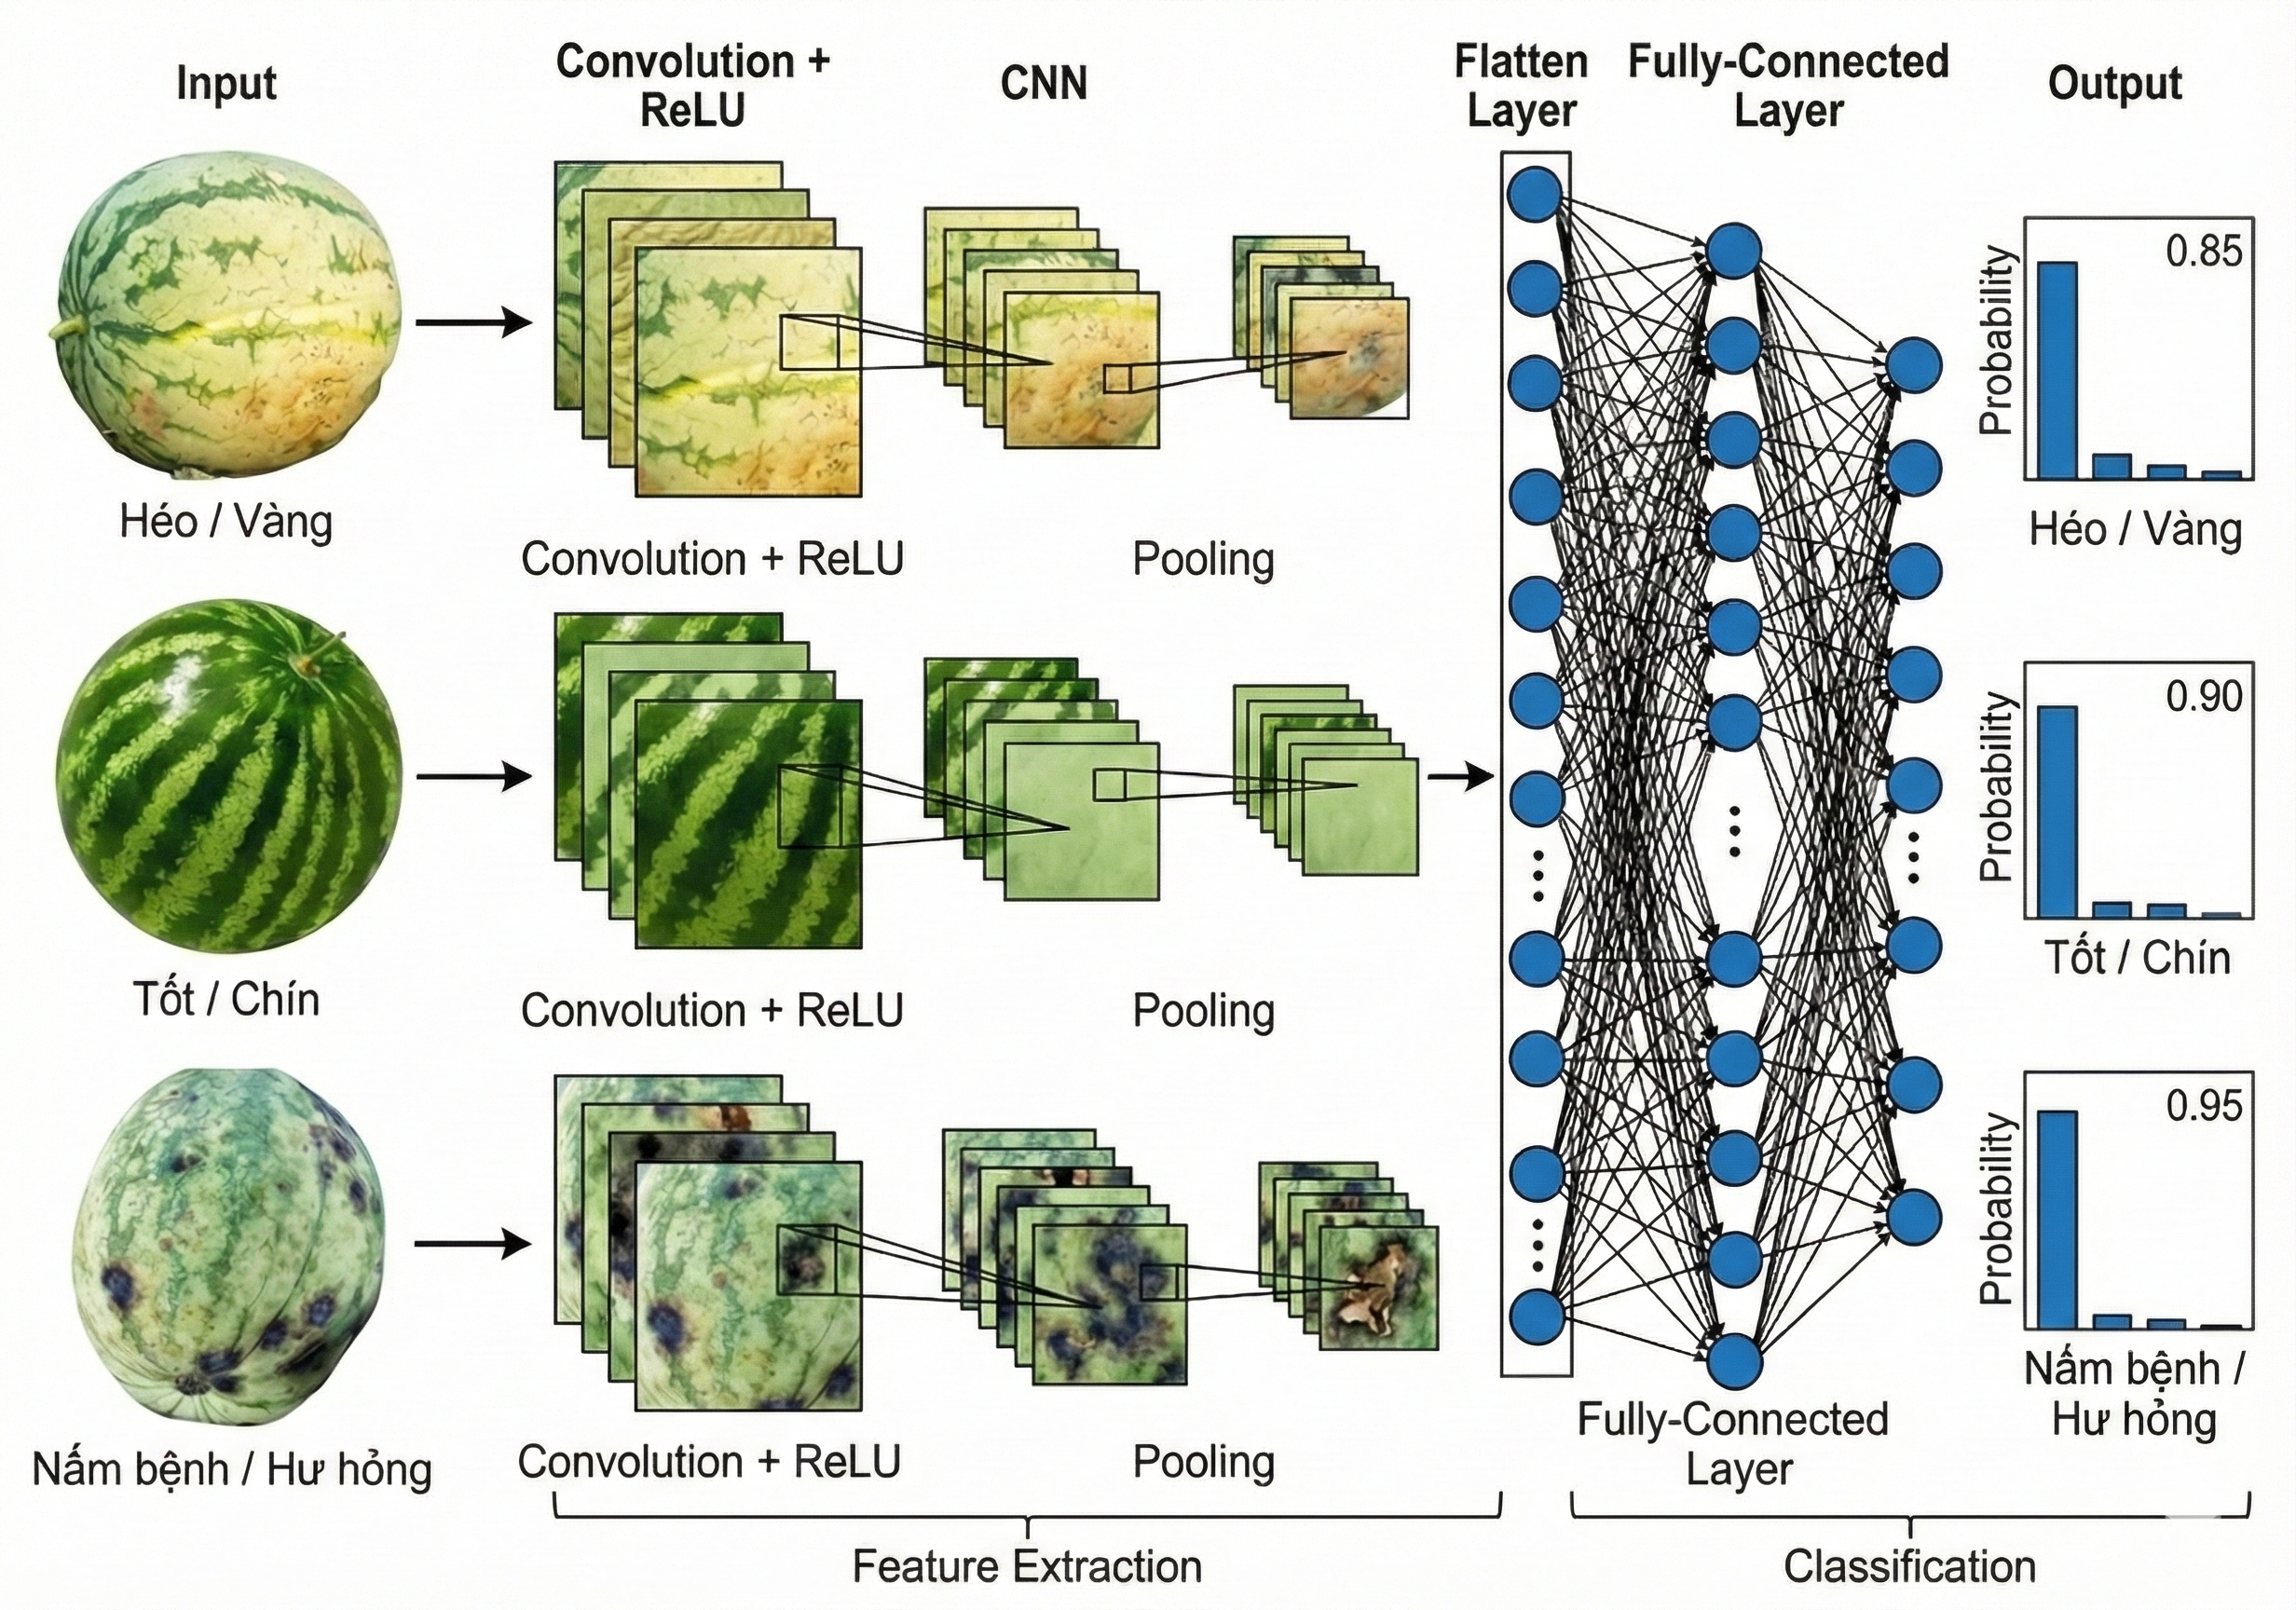
\includegraphics[width=1.0\textwidth]{pictures/cnn_architecture.png}
    \caption{Kiến trúc mạng CNN}
    \label{fig:cnn_arch_1}
\end{figure}


\subsection{Các lớp chính trong CNN}
Nhóm đã thiết kế các lớp CNN như một dây chuyền xử lý ảnh qua nhiều công đoạn:

\begin{table}[H]
    \centering
    \caption{Cấu trúc mạng CNN đề xuất}
    \renewcommand{\arraystretch}{1.3}
    \begin{tabularx}{\textwidth}{|l|X|l|}
        \hline
        \textbf{Lớp} & \textbf{Chức năng} & \textbf{Tham số} \\
        \hline
        Convolutional & Trích xuất đặc trưng cục bộ & 32, 64, 128 filters \\
        \hline
        Activation & Thêm tính phi tuyến ($f(x) = \max(0, x)$) & ReLU \\
        \hline
        Pooling & Giảm kích thước, giữ đặc trưng quan trọng & MaxPooling 2$\times$2 \\
        \hline
        Flatten & Chuyển tensor 2D thành vector 1D & Trước lớp Dense \\
        \hline
        Dense & Kết hợp đặc trưng để phân loại & 128 neurons \\
        \hline
        Softmax & Chuyển output thành xác suất & 3 classes \\
        \hline
    \end{tabularx}
\end{table}

\subsection{Quá trình huấn luyện}
\begin{itemize}
    \item \textbf{Hàm mất mát (Loss Function):} Categorical Cross-Entropy.
    \item \textbf{Thuật toán tối ưu:} Adam Optimizer với learning rate = 0.001.
\end{itemize}

\begin{figure}[H]
    \centering
    \includegraphics[width=1.0\textwidth]{pictures/training_metrics.png}
    \caption{Biểu đồ quá trình huấn luyện (Accuracy và Loss)}
    \label{fig:training_metrics}
\end{figure}

\begin{table}[H]
    \centering
    \caption{Các metrics đánh giá mô hình}
    \renewcommand{\arraystretch}{1.3}
    \begin{tabularx}{\textwidth}{|l|l|X|}
        \hline
        \textbf{Metric} & \textbf{Công thức} & \textbf{Ý nghĩa} \\
        \hline
        Accuracy & (TP + TN) / Total & Tỷ lệ dự đoán đúng trên tổng số mẫu \\
        \hline
        Precision & TP / (TP + FP) & Độ chính xác của các dự đoán dương tính \\
        \hline
        Recall & TP / (TP + FN) & Khả năng phát hiện đúng các mẫu dương tính \\
        \hline
    \end{tabularx}
\end{table}

\section{Lập trình kéo thả Blockly}

\subsection{Giới thiệu Blockly}
Blockly là thư viện JavaScript mã nguồn mở do Google phát triển, cho phép tạo giao diện lập trình trực quan bằng cách kéo thả các khối lệnh như xếp LEGO \cite{google2023}. Thay vì viết code phức tạp, người dùng chỉ cần kéo các khối lệnh và ghép chúng lại với nhau.

\begin{figure}[H]
    \centering
    \includegraphics[width=1.0\textwidth]{pictures/mophong.png}
    \caption{Giao diện lập trình kéo thả Blockly}
    \label{fig:blockly_interface}
\end{figure}

% 

\subsection{Ưu điểm của Blockly}
\begin{table}[H]
    \centering
    \caption{Ưu điểm của lập trình kéo thả}
    \renewcommand{\arraystretch}{1.3}
    \begin{tabularx}{\textwidth}{|l|X|X|}
        \hline
        \textbf{Đặc điểm} & \textbf{Lợi ích} & \textbf{Áp dụng trong đề tài} \\
        \hline
        Trực quan & Không cần nhớ cú pháp & Người nông dân dễ tiếp cận \\
        \hline
        Ngăn lỗi & Các khối chỉ ghép được khi hợp lệ & Giảm lỗi khi tạo kịch bản \\
        \hline
        Đa ngôn ngữ & Xuất code ra Python, JS & Tích hợp với backend Flask \\
        \hline
    \end{tabularx}
\end{table}

\subsection{Các khối lệnh tùy chỉnh}
\begin{itemize}
    \item \textbf{Khi bắt đầu:} Điểm khởi đầu chương trình.
    \item \textbf{Di chuyển trục [X/Y/Z]:} Điều khiển motor di chuyển.
    \item \textbf{Bật/Tắt Relay:} Điều khiển van hút.
    \item \textbf{Về Home:} Đưa cánh tay về vị trí gốc.
    \item \textbf{Nếu nhãn là [...]:} Kiểm tra kết quả phân loại từ AI.
\end{itemize}

\section{Chatbot AI trong nông nghiệp}

\subsection{Xu hướng ứng dụng}
Theo báo cáo của MarketsandMarkets \cite{markets2023}, thị trường AI trong nông nghiệp dự kiến đạt 4.7 tỷ USD vào năm 2028. Chatbot AI đang nổi lên như công cụ hỗ trợ nông dân tiếp cận công nghệ một cách tự nhiên nhất.

\begin{figure}[H]
    \centering
    \includegraphics[width=0.6\textwidth]{pictures/minh_hoa_app.png}
    \caption{Giao diện Chatbot AI trên ứng dụng di động}
    \label{fig:chatbot_app}
\end{figure}

\subsection{Mô hình ngôn ngữ lớn (LLM)}
Hệ thống sử dụng Groq API với model GPT-OSS 120B \cite{groq2024}:

\begin{table}[H]
    \centering
    \caption{Thông số mô hình LLM}
    \renewcommand{\arraystretch}{1.3}
    \begin{tabularx}{\textwidth}{|l|X|}
        \hline
        \textbf{Đặc điểm} & \textbf{Thông số} \\
        \hline
        Model & GPT-OSS 120B \\
        \hline
        Context Window & 128,000 tokens \\
        \hline
        Tốc độ xử lý & >500 tokens/giây (Groq LPU) \\
        \hline
        Ngôn ngữ & Hỗ trợ tiếng Việt \\
        \hline
    \end{tabularx}
\end{table}

\subsection{Các tính năng Chatbot}
\begin{table}[H]
    \centering
    \caption{Các tính năng chính của Chatbot}
    \renewcommand{\arraystretch}{1.3}
    \begin{tabularx}{\textwidth}{|l|X|X|}
        \hline
        \textbf{Tính năng} & \textbf{Ví dụ câu hỏi} & \textbf{Phản hồi mẫu} \\
        \hline
        Thống kê & "Hôm nay phân loại được bao nhiêu?" & "Hôm nay: 523 quả (312 Premium, 156 Second, 55 Defective)" \\
        \hline
        Cảnh báo & "Có vấn đề gì không?" & "Tỷ lệ dưa lỗi tăng 15\% so với hôm qua" \\
        \hline
        Hướng dẫn & "Làm sao tạo kịch bản mới?" & "Vào tab Blockly, kéo khối 'Bắt đầu'..." \\
        \hline
        Báo cáo & "Tổng hợp tuần này" & "Tuần này: 3,245 quả Premium, giá trị ~48.6 triệu VNĐ" \\
        \hline
    \end{tabularx}
\end{table}

\section{Giao thức truyền thông}

\subsection{Serial Communication (UART)}
Đây là giao thức truyền thông nối tiếp giữa máy tính và Arduino - "ngôn ngữ" để máy tính ra lệnh cho robot:

\begin{table}[H]
    \centering
    \caption{Thông số giao tiếp Serial}
    \renewcommand{\arraystretch}{1.3}
    \begin{tabularx}{\textwidth}{|l|c|X|}
        \hline
        \textbf{Tham số} & \textbf{Giá trị} & \textbf{Mô tả} \\
        \hline
        Baud rate & 115200 bps & Tốc độ truyền dữ liệu \\
        \hline
        Data bits & 8 & Số bit dữ liệu \\
        \hline
        Stop bits & 1 & Bit kết thúc \\
        \hline
        Parity & None & Không kiểm tra chẵn lẻ \\
        \hline
    \end{tabularx}
\end{table}

Định dạng lệnh điều khiển:
\begin{itemize}
    \item \texttt{M [dirX] [dirY] [dirZ] [duration] [speed]} - Di chuyển
    \item \texttt{R [state]} - Điều khiển Relay
    \item \texttt{H} - Về Home Z
    \item \texttt{HX} - Về Home X
    \item \texttt{C} - Kiểm tra cảm biến
\end{itemize}

\subsection{WebSocket}
Giao thức full-duplex cho phép truyền dữ liệu hai chiều thời gian thực giữa Server (Flask) và Client (Web/Mobile) \cite{websocket_mdn}. Các sự kiện chính: \texttt{classification\_result}, \texttt{robot\_status}, \texttt{error\_alert}.

\subsection{REST API}
\begin{table}[H]
    \centering
    \caption{Danh sách API Endpoints}
    \renewcommand{\arraystretch}{1.3}
    \begin{tabularx}{\textwidth}{|l|c|X|}
        \hline
        \textbf{Endpoint} & \textbf{Method} & \textbf{Chức năng} \\
        \hline
        /api/classify & POST & Phân loại ảnh dưa hấu \\
        \hline
        /api/robot/move & POST & Điều khiển robot thủ công \\
        \hline
        /api/stats & GET & Lấy dữ liệu thống kê \\
        \hline
    \end{tabularx}
\end{table}

\section{Vai trò và ứng dụng của cánh tay robot}

\subsection{Vai trò trong công nghiệp hiện đại}
Cánh tay robot đóng vai trò then chốt trong cuộc cách mạng công nghiệp 4.0, mang lại những lợi ích vượt trội:

\begin{table}[H]
    \centering
    \caption{Vai trò của robot trong công nghiệp}
    \renewcommand{\arraystretch}{1.3}
    \begin{tabularx}{\textwidth}{|l|X|X|}
        \hline
        \textbf{Vai trò} & \textbf{Mô tả} & \textbf{Ví dụ ứng dụng} \\
        \hline
        \textbf{Tăng năng suất} & Hoạt động 24/7 không mệt mỏi & Dây chuyền lắp ráp ô tô \\
        \hline
        \textbf{Đảm bảo chất lượng} & Độ chính xác cao, ổn định & Hàn điểm, phun sơn \\
        \hline
        \textbf{Giảm chi phí} & Tiết kiệm nhân công lâu dài & Đóng gói, phân loại \\
        \hline
        \textbf{An toàn lao động} & Thay thế con người trong môi trường nguy hiểm & Xử lý hóa chất, nhiệt độ cao \\
        \hline
        \textbf{Linh hoạt} & Dễ lập trình lại cho tác vụ mới & Sản xuất đa dạng sản phẩm \\
        \hline
    \end{tabularx}
\end{table}

\subsection{Ứng dụng trong nông nghiệp}
Trong lĩnh vực nông nghiệp, cánh tay robot ngày càng được ứng dụng rộng rãi:

\begin{table}[H]
    \centering
    \caption{Ứng dụng robot trong nông nghiệp}
    \renewcommand{\arraystretch}{1.3}
    \begin{tabularx}{\textwidth}{|l|X|X|}
        \hline
        \textbf{Ứng dụng} & \textbf{Mô tả} & \textbf{Lợi ích} \\
        \hline
        Thu hoạch trái cây & Nhận diện và hái quả chín & Giảm hao hụt, tăng tốc độ \\
        \hline
        Phân loại nông sản & Phân loại theo kích thước, chất lượng & Chuẩn hóa sản phẩm xuất khẩu \\
        \hline
        Đóng gói & Xếp sản phẩm vào thùng/khay & Tăng năng suất đóng gói \\
        \hline
        Gieo trồng & Gieo hạt chính xác & Tiết kiệm giống, tăng tỷ lệ nảy mầm \\
        \hline
        Phun thuốc & Phun thuốc BVTV chính xác & Giảm lượng thuốc, bảo vệ môi trường \\
        \hline
    \end{tabularx}
\end{table}

\textbf{Áp dụng trong đề tài:} Hệ thống sử dụng cánh tay robot để phân loại dưa hấu - một ứng dụng thực tiễn giúp nâng cao giá trị nông sản Việt Nam.

\section{Thách thức và tương lai}

\subsection{Những thách thức hiện tại}
\begin{table}[H]
    \centering
    \caption{Thách thức của robot nông nghiệp}
    \renewcommand{\arraystretch}{1.3}
    \begin{tabularx}{\textwidth}{|X|X|}
        \hline
        \textbf{Thách thức} & \textbf{Hướng giải quyết} \\
        \hline
        Chi phí đầu tư cao & Phát triển robot giá rẻ, mã nguồn mở \\
        \hline
        Yêu cầu kỹ thuật cao & Giao diện đơn giản hóa (như Blockly) \\
        \hline
        Thiếu linh hoạt & Tích hợp AI và Computer Vision \\
        \hline
    \end{tabularx}
\end{table}

\subsection{Xu hướng tương lai}
\begin{enumerate}
    \item \textbf{Robot cộng tác (Cobot):} Làm việc an toàn bên cạnh con người, không cần rào chắn.
    \item \textbf{Tích hợp AI:} Tự học và thích ứng với môi trường, tự điều chỉnh khi gặp lỗi.
    \item \textbf{Robot di động (AMR):} Kết hợp cánh tay với xe tự hành, linh hoạt di chuyển trong nhà máy.
    \item \textbf{Digital Twin:} Mô phỏng robot trên máy tính trước khi triển khai thực tế.
    \item \textbf{Robot-as-a-Service (RaaS):} Thuê robot theo tháng thay vì mua, giảm chi phí đầu tư ban đầu.
\end{enumerate}

\subsection{Đóng góp của đề tài}
Đề tài này đóng góp vào việc giải quyết một số thách thức:

\begin{table}[H]
    \centering
    \caption{Đóng góp của đề tài}
    \renewcommand{\arraystretch}{1.3}
    \begin{tabularx}{\textwidth}{|l|X|}
        \hline
        \textbf{Thách thức} & \textbf{Giải pháp của đề tài} \\
        \hline
        Chi phí cao & Sử dụng linh kiện phổ thông, chi phí < 50 triệu VNĐ \\
        \hline
        Yêu cầu kỹ thuật & Giao diện Blockly kéo thả, không cần biết code \\
        \hline
        Thiếu linh hoạt & Tích hợp CNN để nhận diện đa dạng loại dưa \\
        \hline
        Khó tiếp cận & Chatbot AI hỗ trợ bằng tiếng Việt tự nhiên \\
        \hline
    \end{tabularx}
\end{table}

% ========================= CHƯƠNG 3 =========================
\chapter{TRÌNH BÀY SẢN PHẨM}

Chương này trình bày chi tiết quá trình xây dựng sản phẩm, từ nguyên liệu, dụng cụ cho đến các bước thực hiện cụ thể.

\section{Nguyên liệu và dụng cụ chế tạo}

\subsection{Tổng quan kiến trúc hệ thống}
Hệ thống được thiết kế theo kiến trúc 3 tầng, tách biệt rõ ràng giữa phần cứng, backend và giao diện người dùng.

\begin{center}
    \begin{figure}[H]
    \centering
    \includegraphics[width=0.65\textwidth]{pictures/so_do_3_tang.pdf}
    \caption{Sơ đồ kiến trúc hệ thống 3 tầng}
    \label{fig:system_arch}
\end{figure}
\end{center}

\textbf{Luồng hoạt động chính:}
Khi hệ thống hoạt động, dữ liệu sẽ đi theo luồng sau:
\begin{enumerate}
    \item \textbf{Camera} chụp ảnh dưa hấu $\rightarrow$ gửi lên \textbf{Backend}.
    \item \textbf{ML Controller} phân loại ảnh $\rightarrow$ trả về nhãn (Premium/Second/Defective).
    \item \textbf{Script Executor} đọc kịch bản Blockly $\rightarrow$ gửi lệnh xuống \textbf{Arduino}.
    \item \textbf{Arduino} điều khiển \textbf{Robot} di chuyển đến vị trí tương ứng.
    \item \textbf{Relay} bật/tắt bơm hút $\rightarrow$ gắp và thả dưa vào thùng đúng.
    \item \textbf{WebSocket} cập nhật trạng thái real-time lên \textbf{Web/Mobile}.
\end{enumerate}

\subsection{Danh sách linh kiện}

\textbf{A. Module điều khiển:}
\begin{table}[H]
    \centering
    \caption{Danh sách module điều khiển}
    \renewcommand{\arraystretch}{1.3}
    \begin{tabularx}{\textwidth}{|c|X|c|X|}
        \hline
        \textbf{STT} & \textbf{Linh kiện} & \textbf{SL} & \textbf{Chức năng} \\
        \hline
        1 & Arduino Uno R3 & 1 & Vi điều khiển chính \\
        \hline
        2 & CNC Shield V3 & 1 & Board mở rộng điều khiển motor \\
        \hline
        3 & Driver A4988 & 3 & Điều khiển động cơ bước \\
        \hline
        4 & Nguồn 12V 5A & 1 & Cấp nguồn cho motor và relay \\
        \hline
        5 & Biến áp 12V $\rightarrow$ 24V & 1 & Tăng áp cho máy bơm \\
        \hline
    \end{tabularx}
\end{table}

\textbf{B. Cơ cấu chấp hành:}
\begin{table}[H]
    \centering
    \caption{Danh sách cơ cấu chấp hành}
    \renewcommand{\arraystretch}{1.3}
    \begin{tabularx}{\textwidth}{|c|X|c|X|}
        \hline
        \textbf{STT} & \textbf{Linh kiện} & \textbf{SL} & \textbf{Chức năng} \\
        \hline
        1 & Động cơ bước NEMA 17 & 3 & Truyền động các khớp \\
        \hline
        2 & Puly GT2 20 răng & 3 & Gắn trục motor \\
        \hline
        3 & Dây đai GT2 200mm & 3 & Truyền động (vòng kín) \\
        \hline
        4 & Máy bơm chân không 24V & 1 & Tạo lực hút \\
        \hline
        5 & Giác hút (Suction Cup) & 1 & Gắp dưa hấu \\
        \hline
        6 & Relay Module 12V & 1 & Đóng/ngắt bơm \\
        \hline
    \end{tabularx}
\end{table}

\textbf{C. Cảm biến và công tắc:}
\begin{table}[H]
    \centering
    \caption{Danh sách cảm biến và công tắc}
    \renewcommand{\arraystretch}{1.3}
    \begin{tabularx}{\textwidth}{|c|X|c|X|}
        \hline
        \textbf{STT} & \textbf{Linh kiện} & \textbf{SL} & \textbf{Chức năng} \\
        \hline
        1 & Công tắc hành trình & 2 & Xác định vị trí Home (X, Z) \\
        \hline
        2 & Cảm biến hồng ngoại & 2 & Báo thùng đầy (Loại 1, Loại 2) \\
        \hline
        3 & Nút nhấn & 1 & Nút bấm hành động (A2) \\
        \hline
        4 & Webcam USB & 1 & Thu nhận hình ảnh \\
        \hline
    \end{tabularx}
\end{table}

\textbf{D. Tụ điện (Lọc nhiễu - Rất quan trọng):}
\begin{table}[H]
    \centering
    \caption{Danh sách tụ điện}
    \renewcommand{\arraystretch}{1.3}
    \begin{tabularx}{\textwidth}{|c|l|l|c|X|}
        \hline
        \textbf{STT} & \textbf{Loại tụ} & \textbf{Thông số} & \textbf{SL} & \textbf{Vị trí lắp} \\
        \hline
        1 & Tụ hóa & 100µF / 25V & 3 & Nguồn mỗi driver A4988 \\
        \hline
        2 & Tụ hóa & 470µF / 25V & 2 & Đầu ra nguồn 5V tổng \\
        \hline
        3 & Tụ gốm & 104 (100nF) & 10 & VCC-GND cảm biến IR \\
        \hline
    \end{tabularx}
\end{table}
\textit{Lưu ý: Môi trường có động cơ bước gây nhiễu nặng, tụ điện là bắt buộc để hệ thống hoạt động ổn định!}

\textbf{E. Vòng bi (Bearings):}
\begin{table}[H]
    \centering
    \caption{Danh sách vòng bi}
    \renewcommand{\arraystretch}{1.3}
    \begin{tabularx}{\textwidth}{|c|l|c|X|}
        \hline
        \textbf{STT} & \textbf{Loại} & \textbf{SL} & \textbf{Vị trí sử dụng} \\
        \hline
        1 & F686ZZ & 12 & Khớp vai, định vị tâm \\
        \hline
        2 & F624ZZ & 8 & Khớp nối thanh truyền \\
        \hline
        3 & 51105 & 2 & Đế xoay (chịu lực dọc trục) \\
        \hline
    \end{tabularx}
\end{table}

\textbf{F. Ốc vít:}
\begin{table}[H]
    \centering
    \caption{Danh sách ốc vít}
    \renewcommand{\arraystretch}{1.3}
    \begin{tabularx}{\textwidth}{|l|l|c|X|}
        \hline
        \textbf{Loại} & \textbf{Kích thước} & \textbf{SL} & \textbf{Vị trí} \\
        \hline
        M2 & 10mm + đai ốc & 10 bộ & Gắn công tắc hành trình \\
        \hline
        M3 & 6mm & 50 & Gắn motor, các chi tiết nhỏ \\
        \hline
        M4 & 10mm, 16mm, 20mm & 25 bộ & Kết nối khung, thanh truyền \\
        \hline
        M6 & 50mm + đai ốc & 2 & Trục xoay chính \\
        \hline
    \end{tabularx}
\end{table}

\subsection{Thiết kế khung robot (in 3D)}
Toàn bộ khung robot được in 3D bằng nhựa PLA/PETG, chia thành các cụm lắp ráp:

\textbf{A. Đế xoay (Base) - Chịu tải toàn bộ robot:}

\begin{figure}[H]
    \centering
    \includegraphics[width=0.8\textwidth]{pictures/base.png}
    \caption{Thiết kế đế xoay (Base)}
    \label{fig:base}
\end{figure}
\begin{itemize}
    \item \textbf{base\_ring:} Vòng đế ngoài cùng.
    \item \textbf{socket:} Đế giữ bạc đạn chính.
    \item \textbf{base:} Phần đế tam giác.
    \item \textbf{rotategear:} Bánh răng lớn để xoay đế.
\end{itemize}
\textit{Lắp ráp:} Bạc đạn 51105 (chịu lực nén) + F686ZZ (định vị tâm) + 1 công tắc hành trình.

\textbf{B. Thân robot (Body) - Chứa động cơ:}

\begin{figure}[H]
    \centering
    \includegraphics[width=0.8\textwidth]{pictures/Body.png}
    \caption{Thiết kế thân robot (Body)}
    \label{fig:body}
\end{figure}
\begin{itemize}
    \item \textbf{body\_base:} Đế thân chính.
    \item \textbf{steppers:} Khung giữ động cơ.
    \item \textbf{upper\_motor, lower\_motor:} Gá motor trên và dưới.
    \item \textbf{endstop:} Gá công tắc hành trình.
\end{itemize}
\textit{Lắp ráp:} 2 động cơ NEMA 17 + 2 puly GT2 + 2 công tắc hành trình.

\textbf{C. Hệ thống cánh tay (Arms):}

\begin{figure}[H]
    \centering
    \includegraphics[width=0.8\textwidth]{pictures/Arms.png}
    \caption{Hệ thống cánh tay (Arms)}
    \label{fig:arms}
\end{figure}
\begin{itemize}
    \item \textbf{lever:} Đòn bẩy (cho cánh tay trên).
    \item \textbf{lowershank:} Cánh tay dưới.
    \item \textbf{Bánh răng in 3D:} Truyền động từ motor.
\end{itemize}
\textit{Lắp ráp:} Dây đai GT2 200mm + Bạc đạn F686ZZ tại khớp vai.

\textbf{D. Hệ thống thanh truyền song song (Linkage):}

\begin{figure}[H]
    \centering
    \includegraphics[width=0.8\textwidth]{pictures/Linkage.png}
    \caption{Hệ thống thanh truyền song song (Linkage)}
    \label{fig:linkage}
\end{figure}
\begin{itemize}
    \item \textbf{triplate:} Tấm tam giác nối thân và thanh truyền.
    \item \textbf{pleuel:} Thanh truyền dài.
    \item \textbf{pleuel\_bend\_lower:} Thanh truyền cong.
    \item \textbf{upper\_shank:} Cánh tay trên cùng.
\end{itemize}
\textit{Lắp ráp:} Bạc đạn F624ZZ + Ốc M4 16mm, 20mm.

\subsection{Sơ đồ kết nối điện}

\textbf{A. Sơ đồ tổng quan hệ thống điện:}
\begin{center}
    \begin{figure}[H]
    \centering
    \includegraphics[width=1.0\textwidth]{pictures/electrical_overview.png}
    \caption{Sơ đồ tổng quan hệ thống điện}
    \label{fig:electrical_overview}
\end{figure}
\end{center}

\textbf{B. Chi tiết kết nối Arduino UNO $\leftrightarrow$ CNC Shield V3:}
\begin{table}[H]
    \centering
    \caption{Kết nối Arduino và CNC Shield}
    \renewcommand{\arraystretch}{1.3}
    \begin{tabularx}{\textwidth}{|c|c|X|}
        \hline
        \textbf{Chân Arduino} & \textbf{Chân CNC Shield} & \textbf{Chức năng} \\
        \hline
        D2, D3, D4 & X.STEP, Y.STEP, Z.STEP & Xung bước Motor X, Y, Z \\
        \hline
        D5, D6, D7 & X.DIR, Y.DIR, Z.DIR & Hướng Motor X, Y, Z \\
        \hline
        D8 & EN & Enable tất cả driver \\
        \hline
        D9 & Pin 7 (Y+) & IR Sensor 1 \\
        \hline
        D10 & Pin 6 (X+) & IR Sensor 2 \\
        \hline
        D12 & SpnEn & Limit Switch Z (NO$\rightarrow$C) \\
        \hline
        D13 & SpnDir & Limit Switch X (NO$\rightarrow$C) \\
        \hline
        A2 & Resume & Nút nhấn (2Pin Push Switch) \\
        \hline
    \end{tabularx}
\end{table}

\textbf{C. Chi tiết kết nối các thành phần:}
\begin{itemize}
    \item \textbf{Stepper Motors:} Kết nối vào các chân X, Y, Z trên CNC Shield (thứ tự dây: D, B, C, A).
    \item \textbf{Relay 12V:}
    \begin{itemize}
        \item DC+, DC-: Nối vào nguồn 12V của CNC Shield.
        \item IN: Nối vào chân Z- của CNC Shield.
        \item COM: Nối vào Air Valve VDD.
        \item NO: Nối vào nguồn 12V.
    \end{itemize}
    \item \textbf{Cảm biến hồng ngoại (IR Sensor):} Nguồn 3.3V, Output nối vào X+ (D10) và Y+ (D9).
    \item \textbf{Công tắc hành trình:} Đấu chân C và NO vào SpnEn (D12) và SpnDir (D13).
\end{itemize}

\textbf{D. Danh sách tụ điện và vị trí lắp:}
\begin{table}[H]
    \centering
    \caption{Chi tiết tụ điện lọc nhiễu}
    \renewcommand{\arraystretch}{1.3}
    \begin{tabularx}{\textwidth}{|c|l|l|c|X|}
        \hline
        \textbf{STT} & \textbf{Loại tụ} & \textbf{Thông số} & \textbf{SL} & \textbf{Vị trí lắp} \\
        \hline
        1 & Tụ hóa & 100µF / 50V & 1 & CNC Shield +VE/-VE (Lọc nguồn chính) \\
        \hline
        2 & Tụ gốm & 104 (100nF) & 3 & Mỗi driver A4988 (Lọc nhiễu cao tần) \\
        \hline
        3 & Tụ gốm & 104 (100nF) & 1 & Relay COM - GND (Lọc nhiễu relay) \\
        \hline
        4 & Tụ hóa & 470µF / 25V & 2 & Terminal Block (Dự trữ năng lượng) \\
        \hline
    \end{tabularx}
\end{table}

\textbf{E. Sơ đồ kết nối cảm biến IR:}
\begin{center}
    \begin{figure}[H]
    \centering
    \includegraphics[width=0.7\textwidth]{pictures/ir_sensor_wiring.png}
    \caption{Sơ đồ kết nối cảm biến IR}
    \label{fig:ir_wiring}
\end{figure}
\end{center}

\textbf{F. Sơ đồ mạch điều khiển Air Pump (5V DC):}
\begin{center}
    \begin{figure}[H]
    \centering
    \includegraphics[width=0.8\textwidth]{pictures/air_pump_circuit.png}
    \caption{Sơ đồ mạch điều khiển Air Pump}
    \label{fig:pump_circuit}
\end{figure}
\end{center}

\textbf{G. Lưu ý quan trọng khi đấu nối:}
\begin{enumerate}
    \item \textbf{Nguồn 12V:} Đi qua Toggle Switch SPST trước khi vào CNC Shield.
    \item \textbf{Tụ lọc nguồn chính:} Tụ hóa 100µF/50V đấu giữa +VE và -VE của CNC Shield.
    \item \textbf{IR Sensor:} Dùng nguồn \textbf{3.3V} từ Multi-channel DC Module (không dùng 5V để tránh nhiễu).
    \item \textbf{Air Pump 5V:} Nguồn từ Step Down LM2596 (12V$\rightarrow$5V), được điều khiển qua Relay.
\end{enumerate}

\section{Các bước thực hiện}

\subsection{Xây dựng phần mềm Backend}

\textbf{A. Cấu trúc thư mục:}
\begin{figure}[H]
\centering
\begin{verbatim}
project/
|-- arduino_main/           (Mã nguồn Arduino)
|   |-- main.ino
|-- main/                   (Backend Server - Python Flask)
|   |-- app.py
|   |-- config.py
|   |-- controllers/        (Xử lý logic)
|   |-- routes/             (Định nghĩa API)
|   |-- static/             (Frontend: CSS, JS)
|   |-- templates/          (Giao diện Web HTML)
|-- mobile_app/             (Ứng dụng Mobile - React Native)
|   |-- App.js
|   |-- src/
|-- model.savedmodel/       (Mô hình AI)
\end{verbatim}
\caption{Cấu trúc thư mục dự án}
\label{fig:project_structure}
\end{figure}

\textbf{B. Thiết kế API:}

\textit{REST API Endpoints:}
\begin{table}[H]
    \centering
    \caption{REST API Endpoints}
    \renewcommand{\arraystretch}{1.3}
    \begin{tabularx}{\textwidth}{|l|c|X|}
        \hline
        \textbf{Endpoint} & \textbf{Method} & \textbf{Mô tả} \\
        \hline
        /api/classify & POST & Phân loại ảnh (Input: base64 image) \\
        \hline
        /api/robot/move & POST & Di chuyển robot (Input: x, y, z, speed) \\
        \hline
        /api/robot/home & POST & Về vị trí Home \\
        \hline
        /api/relay & POST & Bật/tắt bơm hút \\
        \hline
        /api/scripts & GET/POST & Quản lý kịch bản Blockly \\
        \hline
        /api/stats & GET & Lấy thống kê phân loại \\
        \hline
    \end{tabularx}
\end{table}

\textit{WebSocket Events:}
\begin{itemize}
    \item \textbf{Client $\rightarrow$ Server:} connect, run\_script, stop\_script.
    \item \textbf{Server $\rightarrow$ Client:} script\_progress, classification\_result, robot\_status, error.
\end{itemize}

\textbf{C. Thiết kế Model Machine Learning:}
Kiến trúc CNN được sử dụng bao gồm các lớp Conv2D, ReLU, MaxPool, Flatten, Dense và Dropout.
\begin{center}
    \begin{figure}[H]
    \centering
    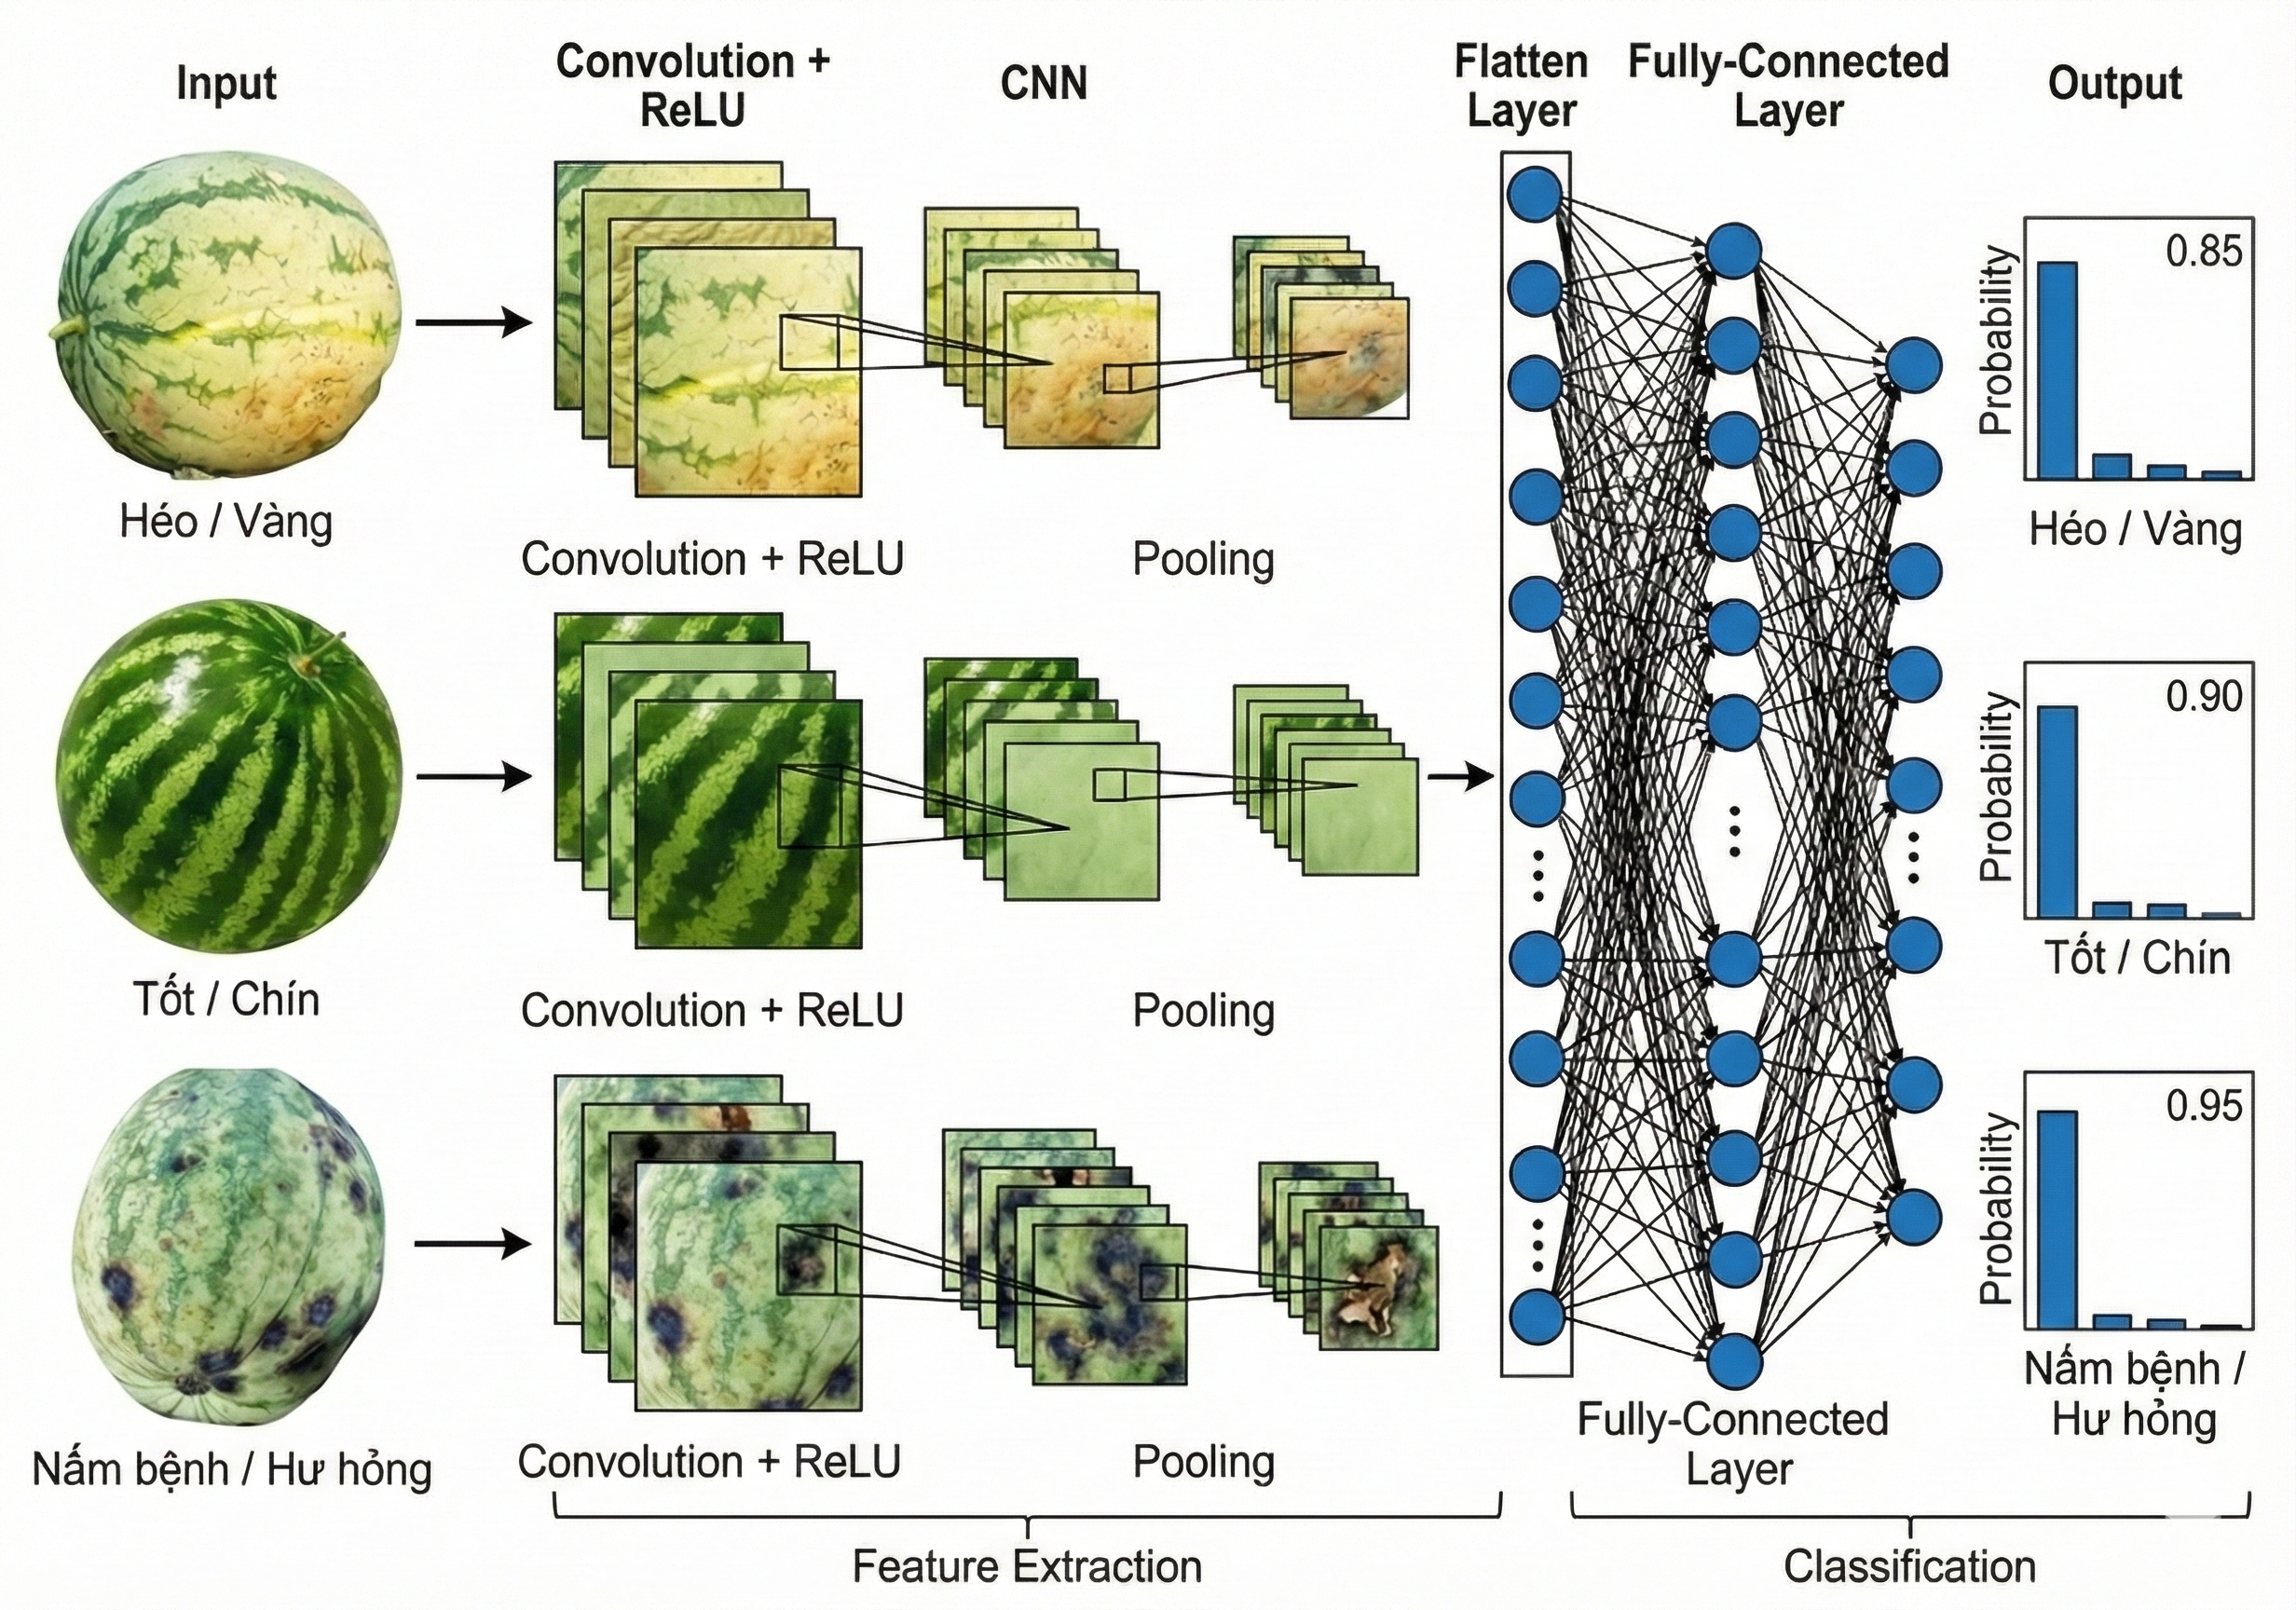
\includegraphics[width=1.0\textwidth]{pictures/cnn_architecture.png}
    \caption{Kiến trúc mạng CNN chi tiết}
    \label{fig:cnn_arch_2}
\end{figure}
\end{center}

\textit{Thông số huấn luyện:}
\begin{itemize}
    \item Dataset: ~3000 ảnh (1000 ảnh/class).
    \item Input size: 224 $\times$ 224 $\times$ 3.
    \item Epochs: 50.
    \item Optimizer: Adam (lr=0.001).
\end{itemize}

\textbf{D. Thiết kế giao diện Blockly:}
Các khối lệnh tùy chỉnh được định nghĩa bằng JavaScript để tạo ra các block như "Di chuyển", "Bật/Tắt bơm", "Nếu nhãn là...".

\subsection{Xây dựng Mobile App}

\textbf{A. Cấu trúc ứng dụng:}
Ứng dụng được xây dựng bằng React Native với cấu trúc gồm các màn hình (screens), components, api client và context management.

\textbf{B. Các màn hình chính:}
\begin{table}[H]
    \centering
    \caption{Các màn hình Mobile App}
    \renewcommand{\arraystretch}{1.3}
    \begin{tabularx}{\textwidth}{|l|X|}
        \hline
        \textbf{Màn hình} & \textbf{Chức năng} \\
        \hline
        ConnectScreen & Kết nối với server qua IP \\
        \hline
        DashboardScreen & Bảng điều khiển, xem thống kê, điều khiển robot \\
        \hline
        HistoryScreen & Xem lịch sử phân loại \\
        \hline
        ChatbotScreen & Trò chuyện với AI (Groq API) \\
        \hline
    \end{tabularx}
\end{table}

\subsection{Lập trình Arduino Firmware}
Firmware Arduino chịu trách nhiệm nhận lệnh G-code hoặc lệnh tùy chỉnh từ Serial, điều khiển các động cơ bước thông qua CNC Shield và đọc tín hiệu từ cảm biến.

\begin{itemize}
    \item \textbf{Xử lý lệnh:} Phân tích chuỗi ký tự nhận được (ví dụ: "M 1 0 0 1000 500").
    \item \textbf{Điều khiển động cơ:} Tạo xung bước (STEP) và hướng (DIR) cho 3 trục X, Y, Z.
    \item \textbf{Homing:} Quy trình về gốc tọa độ sử dụng công tắc hành trình.
    \item \textbf{Relay:} Điều khiển bật/tắt bơm hút.
\end{itemize}

% ========================= CHƯƠNG 4 =========================
\chapter{KẾT LUẬN}

\section{Kết quả đạt được}

\subsection{Về mặt kỹ thuật}
Sau quá trình nghiên cứu và phát triển, hệ thống phân loại dưa hấu đã đạt được những kết quả đáng ghi nhận:

\begin{table}[H]
    \centering
    \caption{Kết quả kỹ thuật đạt được}
    \renewcommand{\arraystretch}{1.3}
    \begin{tabularx}{\textwidth}{|X|c|c|c|}
        \hline
        \textbf{Tiêu chí} & \textbf{Mục tiêu} & \textbf{Kết quả} & \textbf{Đánh giá} \\
        \hline
        Độ chính xác phân loại & $\ge$ 85\% & ~90\% & Đạt \\
        \hline
        Thời gian xử lý/quả & < 5 giây & ~3-4 giây & Đạt \\
        \hline
        Tốc độ di chuyển robot & Ổn định & Mượt mà & Đạt \\
        \hline
        Hệ thống hút chân không & Hút chắc & Hút ổn định & Đạt \\
        \hline
        Giao tiếp Serial & Ổn định & Không mất gói & Đạt \\
        \hline
    \end{tabularx}
\end{table}

\textbf{Chi tiết kết quả:}
\begin{itemize}
    \item \textbf{Cánh tay robot:} Thiết kế Parallel Linkage hoạt động ổn định, vùng làm việc đủ rộng (bán kính ~25cm).
    \item \textbf{AI nhận diện:} Model CNN phân loại tốt 2 loại dưa (Tốt/Xấu), tích hợp Chatbot thông minh.
    \item \textbf{Phần mềm:} Backend Flask và Mobile App hoạt động trơn tru, giao diện Blockly dễ sử dụng.
\end{itemize}

\subsection{Về mặt ứng dụng thực tiễn}
\begin{table}[H]
    \centering
    \caption{Lợi ích thực tiễn}
    \renewcommand{\arraystretch}{1.3}
    \begin{tabularx}{\textwidth}{|l|X|}
        \hline
        \textbf{Đối tượng} & \textbf{Lợi ích mang lại} \\
        \hline
        Nông dân & Giảm công sức, tăng năng suất \\
        \hline
        Thương lái & Đảm bảo chất lượng đồng đều, nâng cao giá trị \\
        \hline
        Người dùng không chuyên & Dễ dàng lập trình qua Blockly \\
        \hline
        Học sinh/Sinh viên & Mô hình học tập trực quan về Robotics/AI \\
        \hline
    \end{tabularx}
\end{table}

\subsection{Về mặt giáo dục và lan tỏa}
\begin{itemize}
    \item \textbf{Mã nguồn mở:} Chia sẻ trên GitHub để cộng đồng tham khảo.
    \item \textbf{Tài liệu đầy đủ:} Hướng dẫn chi tiết từ phần cứng đến phần mềm.
    \item \textbf{Chi phí thấp:} Tổng chi phí linh kiện ~500.000 - 700.000 VNĐ.
    \item \textbf{Khả năng mở rộng:} Thiết kế module hóa, dễ nâng cấp.
\end{itemize}

\section{Hạn chế}

\subsection{Hạn chế về phần cứng}
\begin{table}[H]
    \centering
    \caption{Hạn chế phần cứng}
    \renewcommand{\arraystretch}{1.3}
    \begin{tabularx}{\textwidth}{|l|X|}
        \hline
        \textbf{Hạn chế} & \textbf{Nguyên nhân/Ảnh hưởng} \\
        \hline
        Tải trọng giới hạn & Động cơ NEMA 17 công suất nhỏ (chỉ $\le$ 3kg) \\
        \hline
        Tốc độ chưa cao & Dùng động cơ bước thay vì servo \\
        \hline
        Độ bền khung & Nhựa in 3D có thể biến dạng theo thời gian \\
        \hline
        Giác hút đơn giản & Khó xử lý dưa có bề mặt không đều \\
        \hline
    \end{tabularx}
\end{table}

\subsection{Hạn chế về phần mềm}
\begin{itemize}
    \item \textbf{Bộ dữ liệu nhỏ:} Model CNN chỉ huấn luyện với ~1000 ảnh.
    \item \textbf{Phụ thuộc ánh sáng:} Nhận diện bị ảnh hưởng bởi môi trường.
    \item \textbf{Chưa phân loại đa lớp:} Chỉ phân 2 loại (tốt/xấu).
    \item \textbf{Chatbot cần internet:} Phụ thuộc vào API Groq.
\end{itemize}

\subsection{Hạn chế về triển khai thực tế}
Môi trường thử nghiệm chỉ mới ở phòng lab, chưa triển khai ngoài đồng ruộng. Quy mô thiết kế nhỏ, chưa phù hợp dây chuyền công nghiệp lớn.

\section{Hướng phát triển}

\subsection{Cải tiến ngắn hạn (3-6 tháng)}
\begin{table}[H]
    \centering
    \caption{Đề xuất cải tiến ngắn hạn}
    \renewcommand{\arraystretch}{1.3}
    \begin{tabularx}{\textwidth}{|l|X|}
        \hline
        \textbf{Hạng mục} & \textbf{Giải pháp đề xuất} \\
        \hline
        Tăng tải trọng & Thay NEMA 17 bằng NEMA 23 + driver TB6600 \\
        \hline
        Cải thiện độ bền & Sử dụng nhôm định hình hoặc in 3D Carbon Fiber \\
        \hline
        Mở rộng dữ liệu & Thu thập thêm 5000+ ảnh dưa hấu \\
        \hline
        Bổ sung cảm biến & Thêm cân nặng và đo kích thước \\
        \hline
    \end{tabularx}
\end{table}

\subsection{Phát triển trung hạn (6-12 tháng)}
\begin{itemize}
    \item \textbf{Phân loại đa lớp:} Đặc biệt, Loại 1, Loại 2, Loại 3, Phế phẩm.
    \item \textbf{Tích hợp IoT nâng cao:} Kết nối Farm Management System, đẩy dữ liệu lên cloud.
    \item \textbf{Cải tiến cơ khí:} Băng tải tự động, hệ thống đóng gói.
\end{itemize}

\subsection{Tầm nhìn dài hạn (1-3 năm)}
Xây dựng hệ sinh thái nông nghiệp thông minh với sự kết hợp của Robot phân loại, Robot thu hoạch và Robot chăm sóc.

\begin{center}
    \begin{figure}[H]
    \centering
    \includegraphics[width=0.8\textwidth]{pictures/smart_agri_ecosystem.png}
    \caption{Hệ sinh thái nông nghiệp thông minh}
    \label{fig:ecosystem}
\end{figure}
\end{center}

\subsection{Đóng góp cho cộng đồng}
\begin{table}[H]
    \centering
    \caption{Các hoạt động đóng góp}
    \renewcommand{\arraystretch}{1.3}
    \begin{tabularx}{\textwidth}{|l|X|}
        \hline
        \textbf{Hoạt động} & \textbf{Mục đích} \\
        \hline
        Open-source toàn bộ code & Cộng đồng có thể tham khảo, đóng góp \\
        \hline
        Workshop/Hội thảo & Chia sẻ kinh nghiệm chế tạo robot \\
        \hline
        Tài liệu tiếng Việt & Giúp học sinh, sinh viên tiếp cận công nghệ \\
        \hline
        Hợp tác nghiên cứu & Liên kết với các trường đại học \\
        \hline
    \end{tabularx}
\end{table}

\section{Lời kết}
Đề tài \textbf{"Hệ thống phân loại dưa hấu sử dụng cánh tay robot tích hợp Thị giác máy tính và Chatbot AI"} đã hoàn thành các mục tiêu đề ra ban đầu. Hệ thống không chỉ là một giải pháp kỹ thuật mà còn mang ý nghĩa xã hội sâu sắc – góp phần xóa bỏ khoảng cách giữa công nghệ hiện đại và người nông dân Việt Nam.

Qua quá trình thực hiện đề tài, nhóm đã học hỏi được rất nhiều kiến thức từ cơ khí, điện tử đến lập trình và trí tuệ nhân tạo. Đây là nền tảng quý giá để tiếp tục nghiên cứu và phát triển trong tương lai.

Chúng em xin chân thành cảm ơn quý thầy cô đã hướng dẫn tận tình, các bạn trong nhóm đã cùng nỗ lực, và gia đình đã luôn ủng hộ trong suốt quá trình thực hiện đề tài.

% ========================= PHỤ LỤC =========================
\appendix
\chapter{PHỤ LỤC}

\section{Mã nguồn Arduino (trích)}
\begin{lstlisting}[language=C++, caption={Định nghĩa chân kết nối Arduino}]
// Cac dinh nghia chan ket noi
#define stepPinX 2
#define stepPinY 3  
#define stepPinZ 4
#define dirPinX 5
#define dirPinY 6
#define dirPinZ 7
#define en 8
#define IR_SENSOR_1 9    // Y+ tren CNC Shield
#define IR_SENSOR_2 10   // X+ tren CNC Shield
#define RELAY_PIN 11     // Z- tren CNC Shield
#define Z_LIMIT_PIN 12   // SpnEn
#define X_LIMIT_PIN 13   // SpnDir
#define BTN_ACTION A2    // Resume
\end{lstlisting}

\section{Cấu hình Backend Python (trích)}
\begin{lstlisting}[language=Python, caption={File config.py}]
# config.py
SERIAL_PORT = 'COM3'       # Cong ket noi Arduino
SERIAL_BAUDRATE = 115200   # Toc do truyen
MODEL_PATH = '../model.savedmodel'  # Duong dan mo hinh AI
GROQ_API_KEY = 'gsk_xxxxx'  # API key cho chatbot
\end{lstlisting}

\section{Danh sách khối Blockly}
\begin{table}[H]
    \centering
    \caption{Danh sách khối lệnh Blockly}
    \renewcommand{\arraystretch}{1.3}
    \begin{tabularx}{\textwidth}{|l|X|l|}
        \hline
        \textbf{Khối} & \textbf{Chức năng} & \textbf{Lệnh gửi Arduino} \\
        \hline
        Di chuyển đến XYZ & Điều khiển vị trí & \texttt{MOVE:X,Y,Z} \\
        \hline
        Bật/Tắt bơm & Điều khiển relay & \texttt{PUMP:ON/OFF} \\
        \hline
        Về vị trí Home & Reset vị trí & \texttt{HOME:X/Y/Z} \\
        \hline
        Chờ (ms) & Delay & \texttt{DELAY:time} \\
        \hline
        Phân loại tự động & Kích hoạt AI & \texttt{AUTO:START} \\
        \hline
    \end{tabularx}
\end{table}

\section{Sơ đồ chân CNC Shield V3}
\begin{table}[H]
    \centering
    \caption{Sơ đồ chân CNC Shield V3}
    \renewcommand{\arraystretch}{1.3}
    \begin{tabularx}{\textwidth}{|l|X|l|}
        \hline
        \textbf{Pin Header} & \textbf{Chức năng} & \textbf{Arduino Pin} \\
        \hline
        X.STEP & Xung bước Motor X & D2 \\
        \hline
        Y.STEP & Xung bước Motor Y & D3 \\
        \hline
        Z.STEP & Xung bước Motor Z & D4 \\
        \hline
        X.DIR & Hướng Motor X & D5 \\
        \hline
        Y.DIR & Hướng Motor Y & D6 \\
        \hline
        Z.DIR & Hướng Motor Z & D7 \\
        \hline
        EN & Enable drivers & D8 \\
        \hline
        X+ & Limit/Sensor & D10 \\
        \hline
        Y+ & Limit/Sensor & D9 \\
        \hline
        Z- & Relay control & D11 \\
        \hline
        SpnEn & Limit Z & D12 \\
        \hline
        SpnDir & Limit X & D13 \\
        \hline
        Resume & Button & A2 \\
        \hline
    \end{tabularx}
\end{table}

% ========================= TÀI LIỆU THAM KHẢO =========================
\newpage
\addcontentsline{toc}{chapter}{TÀI LIỆU THAM KHẢO} 

\begin{thebibliography}{99}
    \bibitem{szeliski2022} Szeliski, R. (2022). \textit{Computer Vision: Algorithms and Applications, 2nd Edition}. Springer.
    \bibitem{lecun2015} LeCun, Y., Bengio, Y., \& Hinton, G. (2015). Deep Learning. \textit{Nature}, 521(7553), 436-444.
    \bibitem{siciliano2016} Siciliano, B., \& Khatib, O. (2016). \textit{Springer Handbook of Robotics, 2nd Edition}. Springer.
    \bibitem{craig2018} Craig, J. J. (2018). \textit{Introduction to Robotics: Mechanics and Control, 4th Edition}. Pearson.
    \bibitem{fao2022} FAO (2022). \textit{FAOSTAT - Crops and livestock products}. Food and Agriculture Organization.
    \bibitem{sofri2023} Viện Cây ăn quả Miền Nam - SOFRI (2023). \textit{Báo cáo tình hình sản xuất trái cây vùng ĐBSCL}.
    \bibitem{rauqua2023} Hiệp hội Rau quả Việt Nam (2023). \textit{Báo cáo xuất khẩu rau quả năm 2023}.
    \bibitem{gso2022} Tổng cục Thống kê (2022). \textit{Niên giám thống kê nông nghiệp}.
    \bibitem{ifr2023} International Federation of Robotics - IFR (2023). \textit{World Robotics Report 2023}.
    \bibitem{mckinsey2023} McKinsey \& Company (2023). \textit{Digital Agriculture: The future of farming in Asia}.
    \bibitem{markets2023} MarketsandMarkets (2023). \textit{AI in Agriculture Market - Global Forecast to 2028}.
    \bibitem{arduino_doc} Arduino Documentation. \textit{Arduino Uno Rev3 Datasheet}. \url{https://docs.arduino.cc/hardware/uno-rev3}
    \bibitem{pololu} Pololu. \textit{A4988 Stepper Motor Driver Carrier}. \url{https://www.pololu.com/product/1182}
    \bibitem{ti_lm2596} Texas Instruments. \textit{LM2596 SIMPLE SWITCHER Power Converter Datasheet}.
    \bibitem{esp32} Espressif Systems. \textit{ESP32 Technical Reference Manual}.
    \bibitem{flask} Flask Documentation. \textit{Flask-SocketIO}. \url{https://flask-socketio.readthedocs.io/}
    \bibitem{tensorflow} TensorFlow. \textit{SavedModel Guide}. \url{https://www.tensorflow.org/guide/saved_model}
    \bibitem{reactnative} React Native Documentation. \textit{Getting Started}. \url{https://reactnative.dev/docs/getting-started}
    \bibitem{google2023} Google Developers (2023). \textit{Blockly Developer Documentation}. \url{https://developers.google.com/blockly}
    \bibitem{groq2024} Groq Inc. (2024). \textit{Groq API Documentation}. \url{https://console.groq.com/docs}
    \bibitem{opencv} OpenCV Documentation. \url{https://docs.opencv.org/}
    \bibitem{python} Python Documentation. \url{https://docs.python.org/3/}
    \bibitem{websocket_mdn} MDN Web Docs. \textit{WebSocket API}. \url{https://developer.mozilla.org/en-US/docs/Web/API/WebSocket}
\end{thebibliography}

\end{document}